%%%%%%%%%%%%%%%%%%%%%%%%%%%%%%%%%%%%%%%%%
% Masters/Doctoral Thesis 
% LaTeX Template
% Version 2.5 (27/8/17)
%
% This template was downloaded from:
% http://www.LaTeXTemplates.com
%
% Version 2.x major modifications by:
% Vel (vel@latextemplates.com)
%
% This template is based on a template by:
% Steve Gunn (http://users.ecs.soton.ac.uk/srg/softwaretools/document/templates/)
% Sunil Patel (http://www.sunilpatel.co.uk/thesis-template/)
%
% Template license:
% CC BY-NC-SA 3.0 (http://creativecommons.org/licenses/by-nc-sa/3.0/)
%
%%%%%%%%%%%%%%%%%%%%%%%%%%%%%%%%%%%%%%%%%

%----------------------------------------------------------------------------------------
%	PACKAGES AND OTHER DOCUMENT CONFIGURATIONS
%----------------------------------------------------------------------------------------
\PassOptionsToPackage{table,xcdraw}{xcolor}
\documentclass[
12pt, % The default document font size, options: 10pt, 11pt, 12pt
%oneside, % Two side (alternating margins) for binding by default, uncomment to switch to one side
english, % ngerman for German
singlespacing, % Single line spacing, alternatives: onehalfspacing or doublespacing
%draft, % Uncomment to enable draft mode (no pictures, no links, overfull hboxes indicated)
%nolistspacing, % If the document is onehalfspacing or doublespacing, uncomment this to set spacing in lists to single
%liststotoc, % Uncomment to add the list of figures/tables/etc to the table of contents
%toctotoc, % Uncomment to add the main table of contents to the table of contents
%parskip, % Uncomment to add space between paragraphs
%nohyperref, % Uncomment to not load the hyperref package
headsepline, % Uncomment to get a line under the header
%chapterinoneline, % Uncomment to place the chapter title next to the number on one line
%consistentlayout, % Uncomment to change the layout of the declaration, abstract and acknowledgements pages to match the default layout
]{MastersDoctoralThesis} % The class file specifying the document structure

\usepackage[utf8]{inputenc} % Required for inputting international characters
\usepackage[T1]{fontenc} % Output font encoding for international characters

\usepackage{mathpazo} % Use the Palatino font by default

\usepackage[backend=bibtex,style=authoryear,natbib=true]{biblatex} % Use the bibtex backend with the authoryear citation style (which resembles APA)

\addbibresource{example.bib} % The filename of the bibliography

\usepackage[autostyle=true]{csquotes} % Required to generate language-dependent quotes in the bibliography

\usepackage{amsmath}
\usepackage{mathrsfs}
\usepackage{scrextend}

% For algorithms
\usepackage{algorithm}
%\usepackage{algorithmic}
\usepackage{algpseudocode}
%\usepackage{algpseudocode}
%\usepackage{braket} % needed for \Set

\usepackage{listings}
\usepackage{color}
\usepackage{subfigure}
 
\usepackage{enumitem}

\definecolor{codegreen}{rgb}{0,0.6,0}
\definecolor{codegray}{rgb}{0.5,0.5,0.5}
\definecolor{codepurple}{rgb}{0.58,0,0.82}
\definecolor{backcolour}{rgb}{0.95,0.95,0.92}
 
\lstdefinestyle{mystyle}{
    commentstyle=\color{codegreen},
    keywordstyle=\color{magenta},
    numberstyle=\tiny\color{codegray},
    stringstyle=\color{codepurple},
    basicstyle=\footnotesize,
    breakatwhitespace=false,         
    breaklines=true,                 
    captionpos=b,                    
    keepspaces=true,                 
    numbers=left,                    
    numbersep=5pt,                  
    showspaces=false,                
    showstringspaces=false,
    showtabs=false,                  
    tabsize=2
}
 
\lstset{style=mystyle}

%----------------------------------------------------------------------------------------
%	MARGIN SETTINGS
%----------------------------------------------------------------------------------------

\geometry{
	paper=a4paper, % Change to letterpaper for US letter
	inner=2.5cm, % Inner margin
	outer=3.8cm, % Outer margin
	bindingoffset=.5cm, % Binding offset
	top=1.5cm, % Top margin
	bottom=1.5cm, % Bottom margin
	%showframe, % Uncomment to show how the type block is set on the page
}

%----------------------------------------------------------------------------------------
%	THESIS INFORMATION
%----------------------------------------------------------------------------------------

\thesistitle{Transfer Learning with Generative Adversarial Networks in Reinforcement Learning Tasks} % Your thesis title, this is used in the title and abstract, print it elsewhere with \ttitle
\supervisor{Dr. Timothy \textsc{Hospedales}} % Your supervisor's name, this is used in the title page, print it elsewhere with \supname
\examiner{} % Your examiner's name, this is not currently used anywhere in the template, print it elsewhere with \examname
\degree{Bachelor's of Engineering} % Your degree name, this is used in the title page and abstract, print it elsewhere with \degreename
\author{Giovanni \textsc{Alcantara}} % Your name, this is used in the title page and abstract, print it elsewhere with \authorname
\addresses{} % Your address, this is not currently used anywhere in the template, print it elsewhere with \addressname

\subject{Computer Science} % Your subject area, this is not currently used anywhere in the template, print it elsewhere with \subjectname
\keywords{} % Keywords for your thesis, this is not currently used anywhere in the template, print it elsewhere with \keywordnames
\university{\href{https://www.ed.ac.uk/}{The University of Edinburgh}} % Your university's name and URL, this is used in the title page and abstract, print it elsewhere with \univname
\department{\href{https://www.ed.ac.uk/science-engineering}{College of Science \& Engineering}} % Your department's name and URL, this is used in the title page and abstract, print it elsewhere with \deptname
\group{\href{http://www.inf.ed.ac.uk/}{School of Informatics}} % Your research group's name and URL, this is used in the title page, print it elsewhere with \groupname
\faculty{\href{http://faculty.university.com}{Faculty Name}} % Your faculty's name and URL, this is used in the title page and abstract, print it elsewhere with \facname

\AtBeginDocument{
\hypersetup{pdftitle=\ttitle} % Set the PDF's title to your title
\hypersetup{pdfauthor=\authorname} % Set the PDF's author to your name
\hypersetup{pdfkeywords=\keywordnames} % Set the PDF's keywords to your keywords
}

\begin{document}

\frontmatter % Use roman page numbering style (i, ii, iii, iv...) for the pre-content pages

\pagestyle{plain} % Default to the plain heading style until the thesis style is called for the body content

%----------------------------------------------------------------------------------------
%	TITLE PAGE
%----------------------------------------------------------------------------------------

\begin{titlepage}
\begin{center}

\vspace*{.06\textheight}
{\scshape\LARGE \univname\par}\vspace{1.5cm} % University name
\textsc{\Large Informatics Honors Thesis}\\[0.5cm] % Thesis type

\HRule \\[0.4cm] % Horizontal line
{\huge \bfseries \ttitle\par}\vspace{0.4cm} % Thesis title
\HRule \\[1.5cm] % Horizontal line
 
\begin{minipage}[t]{0.4\textwidth}
\begin{flushleft} \large
\emph{Author:}\\
\href{http://www.giovannialcantara.com}{\authorname} % Author name - remove the \href bracket to remove the link
\end{flushleft}
\end{minipage}
\begin{minipage}[t]{0.4\textwidth}
\begin{flushright} \large
\emph{Supervisor:} \\
\href{https://www.inf.ed.ac.uk/people/staff/Timothy_Hospedales.html}{\supname} % Supervisor name - remove the \href bracket to remove the link  
\end{flushright}
\end{minipage}\\[3cm]

\begin{figure}
\centering

\includegraphics[width=3cm]{Figures/Logo.png} % University/department logo - uncomment to place it
\end{figure}

\vfill

\large \textit{A thesis submitted in fulfilment of the requirements\\ for the degree of \degreename}\\[0.3cm] % University requirement text
\textit{in the}\\[0.4cm]
\groupname\\\deptname\\[2cm] % Research group name and department name
 
\vfill

{\large \today}\\[4cm] % Date
 
\vfill
\end{center}
\end{titlepage}

%----------------------------------------------------------------------------------------
%	DECLARATION PAGE
%----------------------------------------------------------------------------------------

%\begin{declaration}
%\addchaptertocentry{\authorshipname} % Add the declaration to the table of contents
%\noindent I, \authorname, declare that this thesis titled, \enquote{\ttitle} and the work presented in it are my own. I confirm that:
%
%\begin{itemize} 
%\item This work was done wholly or mainly while in candidature for a research degree at this University.
%\item Where any part of this thesis has previously been submitted for a degree or any other qualification at this University or any other institution, this has been clearly stated.
%\item Where I have consulted the published work of others, this is always clearly attributed.
%\item Where I have quoted from the work of others, the source is always given. With the exception of such quotations, this thesis is entirely my own work.
%\item I have acknowledged all main sources of help.
%\item Where the thesis is based on work done by myself jointly with others, I have made clear exactly what was done by others and what I have contributed myself.\\
%\end{itemize}
% 
%\noindent Signed:\\
%\rule[0.5em]{25em}{0.5pt} % This prints a line for the signature
% 
%\noindent Date:\\
%\rule[0.5em]{25em}{0.5pt} % This prints a line to write the date
%\end{declaration}
%
%\cleardoublepage

%----------------------------------------------------------------------------------------
%	QUOTATION PAGE
%----------------------------------------------------------------------------------------

%\vspace*{0.2\textheight}
%
%\noindent\enquote{\itshape Thanks to my solid academic training, today I can write hundreds of words on virtually any topic without possessing a shred of information, which is how I got a good job in journalism.}\bigbreak
%
%\hfill Dave Barry

%----------------------------------------------------------------------------------------
%	ABSTRACT PAGE
%----------------------------------------------------------------------------------------

\begin{abstract}
\addchaptertocentry{\abstractname} % Add the abstract to the table of contents
% TODO: Abstract
\end{abstract}

%----------------------------------------------------------------------------------------
%	ACKNOWLEDGEMENTS
%----------------------------------------------------------------------------------------

\begin{acknowledgements}
\addchaptertocentry{\acknowledgementname} % Add the acknowledgements to the table of contents
%TODO
Lorem ipsum dolor sit amet, consectetur adipiscing elit, sed do eiusmod tempor incididunt ut labore et dolore magna aliqua. Ut enim ad minim veniam, quis nostrud exercitation ullamco laboris nisi ut aliquip ex ea commodo consequat. Duis aute irure dolor in reprehenderit in voluptate velit esse cillum dolore eu fugiat nulla pariatur. Excepteur sint occaecat cupidatat non proident, sunt in culpa qui officia deserunt mollit anim id est laborum.
\end{acknowledgements}

%----------------------------------------------------------------------------------------
%	LIST OF CONTENTS/FIGURES/TABLES PAGES
%----------------------------------------------------------------------------------------

\tableofcontents % Prints the main table of contents
%
%\listoffigures % Prints the list of figures
%
%\listoftables % Prints the list of tables

%----------------------------------------------------------------------------------------
%	SYMBOLS
%----------------------------------------------------------------------------------------

%\begin{symbols}{lll} % Include a list of Symbols (a three column table)
%
%$a$ & distance & \si{\meter} \\
%$P$ & power & \si{\watt} (\si{\joule\per\second}) \\
%%Symbol & Name & Unit \\
%
%\addlinespace % Gap to separate the Roman symbols from the Greek
%
%$\omega$ & angular frequency & \si{\radian} \\
%
%\end{symbols}

%----------------------------------------------------------------------------------------
%	DEDICATION
%----------------------------------------------------------------------------------------

%\dedicatory{For/Dedicated to/To my\ldots} 

%----------------------------------------------------------------------------------------
%	THESIS CONTENT - CHAPTERS
%----------------------------------------------------------------------------------------

\mainmatter % Begin numeric (1,2,3...) page numbering

\pagestyle{thesis} % Return the page headers back to the "thesis" style

% Include the chapters of the thesis as separate files from the Chapters folder
% Uncomment the lines as you write the chapters

% Chapter 1

\chapter{Introduction} % Main chapter title
\label{Chapter1} % For referencing the chapter elsewhere, use \ref{Chapter1} 

%----------------------------------------------------------------------------------------

% Define some commands to keep the formatting separated from the content 
\newcommand{\keyword}[1]{\textbf{#1}}
\newcommand{\tabhead}[1]{\textbf{#1}}
\newcommand{\code}[1]{\texttt{#1}}
\newcommand{\file}[1]{\texttt{\bfseries#1}}
\newcommand{\option}[1]{\texttt{\itshape#1}}

%----------------------------------------------------------------------------------------

\section{Motivation}
\label{motivation}
% - 
% - Improve transferability of reinforcement learning domains
% - Leverage power of neural networks to model and estimate complex systems
% - 

Reinforcement learning is the problem faced by an agent that must learn behaviour through trial-and-error interactions with an environment.

Reinforcement learning as a field has had major successes in the past few years \parencite{tesauro1995temporal, singh2002optimizing, kohl2004policy, ng2006autonomous}, particularly as techniques utilising deep neural networks (DNN) have started permeating the research community. Techniques like Q-network \parencite{mnih2015human}, trust region policy optimisation \parencite{schulman2015trust}, and asynchronous advantage actor-critic (A3C) \parencite{mnih2016asynchronous} helped stemmed an area of research of recent significant importance: deep reinforcement learning (DRL) \parencite{DBLP:journals/corr/abs-1708-05866}.

Traditional reinforcement learning approaches generally lacked scalability, limiting these techniques to fairly low-dimensional problems. These limitations are in terms of memory complexity and computational complexity \parencite{kaelbling1996reinforcement}.

As such, using these usually becomes intractable when modelling real-world systems, due to the many variables and unknowns that are present in such systems \parencite{strehl2006pac}.

As DRL methods rectified some of these issues, new ones started to emerge, particularly limitations inherent to using deep neural networks. Notably, the need to have access to large datasets for training, particularly if in the context of applications that require image processing, such as autonomous vehicle control \parencite{krizhevsky2012imagenet}, has proven to be a critical limitation. 

In real-world reinforcement learning applications, environment observations often rely heavily on computer vision and image processing \parencite{berns1992reinforcement}, which often provide an incomplete picture of the state that the agent is in. In such types of scenario, formally known as partially observable Markov decision processes (POMDP) \parencite{monahan1982state}, not only do we have fragmentary observations, but it is also sometimes prohibitive to build large datasets that DRL requires to train the agent.

In deep learning, one of the ways to circumvent this constraint is \emph{transfer learning}, the ability to leverage models trained in a particular domain on different applications. Transfer learning has proven pivotal in achieving successes in a wide variety of applications, without the need to train expensive models from scratch \parencite{pan2010survey}.

There has been much work in improving transferability of reinforcement learning models, most notably multitask learning \parencite{caruana1998multitask} and curriculum learning \parencite{bengio2009curriculum}, though few methods have tried to bootstrap learning with the use of DNNs.

There are few successes in transferring deep reinforcement learning across domains. Mostly notably, \cite{jaderberg2016reinforcement} introduced a technique to identify, in an unsupervised way, multiple pseudo-reward functions based on all training signals that the agent collected as observations. While doing deep reinforcement learning, therefore, \citeauthor{jaderberg2016reinforcement} would not only try to directly maximise the agent's cumulative reward, but also all the identified extrinsic rewards. There is a potential to use these identified extrinsic rewards in other domains, but this is a backwards way to tackle the problem of transferring behaviour. Here, we would first identify what auxiliary rewards the observations can give, to then reuse them on different task. Also, we have little to no control to guide the unsupervised exploration of auxiliary rewards functions towards a related task that we have the power to define. In fairness, \citeauthor{jaderberg2016reinforcement} introduced auxiliary rewards as a way to speed up reinforcement learning on a single task, rather than aiming to transfer these to related tasks.
%TODO: Add regularization
In our work we provide a general framework that lets us speed up reinforcement learning on unseen tasks in related domains. We do this by training deep learning models over a distribution of optimal policies for different configurations of a task in a certain domain. More specifically, given a distribution of trained policies in variations of an environment, we train two models: a generative model that is able to generate policies for different configurations of a task in a domain, and a discriminative model that is able to tell whether a policy is a good one within this domain. We show how using these models while doing reinforcement learning can speed up learning on new unseen configurations.

The generative model and the discriminative model are trained using deep neural networks in an adversarial architecture also know as a Generative Adversarial Network (GAN), introduced in \cite{goodfellow2014generative}'s seminal work. While this idea was popularised with applications in image synthesis, most notably Deep Convolutional Generative Adversarial Networks \parencite{radford2015unsupervised}, there have been successes using GANs within reinforcement learning.

Specifically, work on generative adversarial imitation learning \parencite{ho2016generative} has shown remarkable speedups in the task of imitating behaviour given expert policies.

\section{Goal}
\label{goal}
Given all these motivations, we can now define the \textbf{final goal of our work}: \\

\begin{addmargin}[3em]{3em}
\emph{Transferring knowledge} obtained with reinforcement learning techniques on certain tasks to similar, unseen tasks, by leveraging the power of \emph{Generative Adversarial Networks} (GANs). In this way, we hope to \emph{achieve shorter training times} and \emph{better rewards} when training models for these \emph{unseen tasks}.
\end{addmargin}

%----------------------------------------------------------------------------------------

\section{Data pipeline}
\label{sec:datapipeline}
In this section we provide a bird's eye view to the whole project by showing a visual schematic of the data pipeline (Figure~\ref{fig:pipeline})

We will be referencing this pipeline schematic throughout the whole report. In fact, as we dive deeper into technical details of each component of the data pipeline, it is critical to take them in the context of the whole pipeline as to justify certain design decisions we make for our experiments.

At this point, it is important to highlight how we achieve the goal we set in the previous subsection (subsection~\ref{goal}) with this data pipeline.

The input to our system is a set of similar tasks that would be traditionally solved with reinforcement learning techniques. What makes these tasks similar is the fact that they where the goal is the same, but the agent operates in different map configurations. We provide more details on the environment in Chapter~\ref{Chapter3}.
We split these tasks into a test set and a training set. We train all of these maps configurations with Q-learning, a reinforcement learning technique to obtain optimal policies. 

Now, what we want to achieve, as per our goal, is:
\begin{enumerate}
	\item train a GAN system to capture the distribution of the policies in the training set,
	\item use the trained GAN to develop a new algorithm that is able to transfer that knowledge to speed up training of tasks in the test set of map configurations,
	\item verify and benchmark that the test policies obtained with the new method are better than the ones trained with traditional Q-learning.
\end{enumerate}

\begin{figure}
\centering
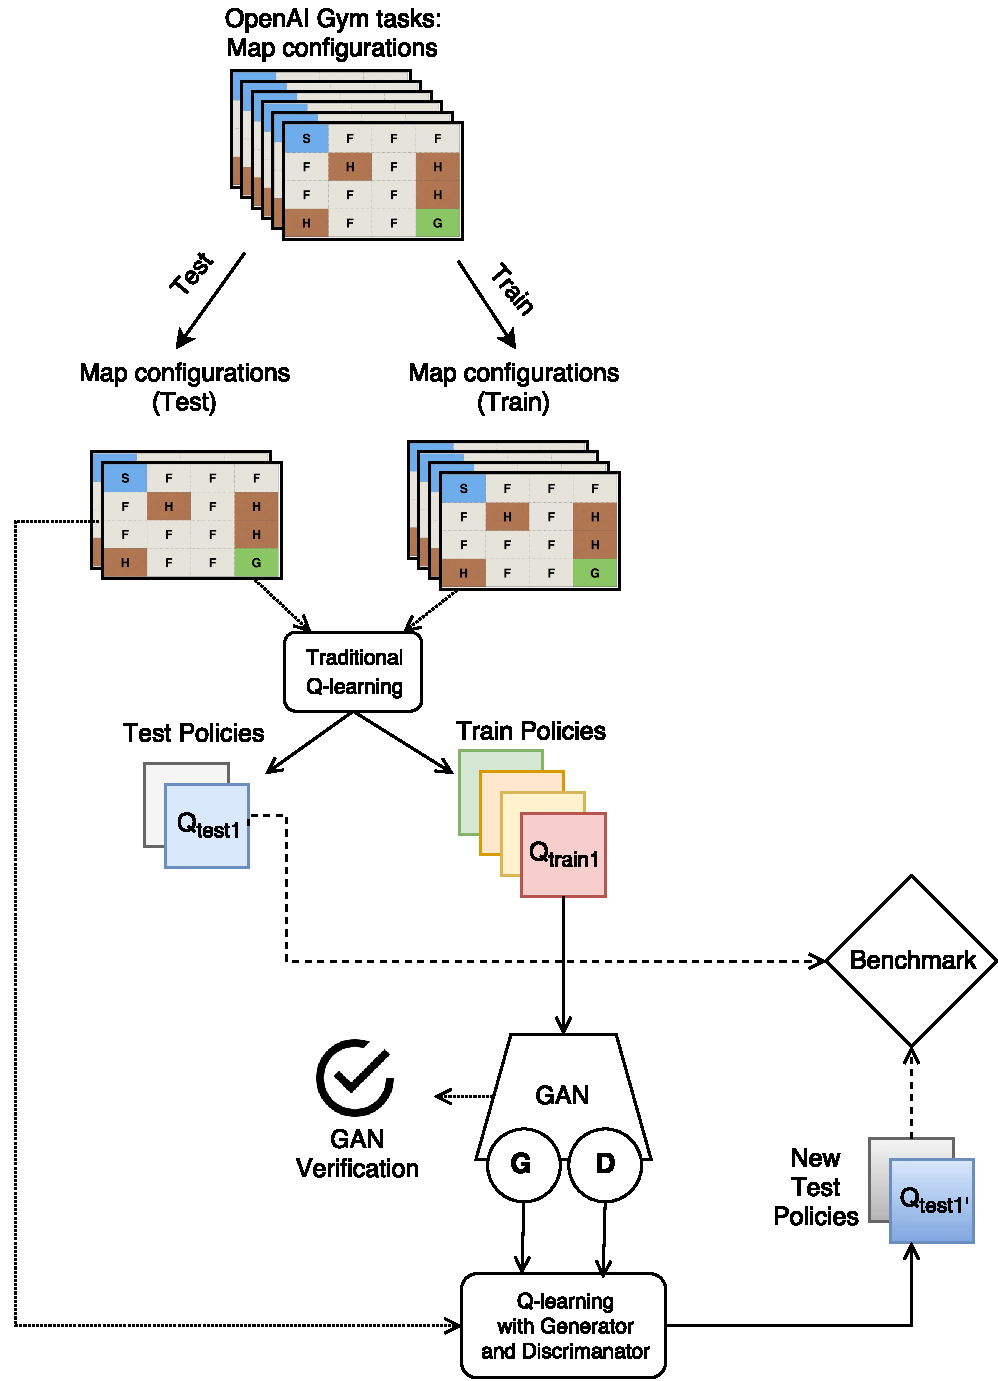
\includegraphics[width=10cm]{Figures/Pipeline}
\caption{The Data Pipeline}
\label{fig:pipeline}
\end{figure}

%----------------------------------------------------------------------------------------

\section{Structure of the report}
Our report is structured in a what that strongly follows each component of the data pipeline outlined in the previous subsection.
% TODO: Finish structure
\begin{itemize}
	\item Chapter~\ref{Chapter2} introduces important background information on reinforcement learning, Markov Decision Processes, Q-learning and Generative Adversarial Networks.
	\item Chapter~\ref{Chapter3} details the environment being used in our experiments.
	\item Chapter~\ref{Chapter4} reports on the process of training policies on all the different tasks with traditional reinforcement learning (Q-learning).
	\item Chapter~\ref{Chapter5} outlines the process of training the GAN given the trained policies in the training set.
	\item Chapter~\ref{Chapter6} describes the new algorithm we develop to speed up learning on unseen tasks.
	\item Chapter
\end{itemize}

%----------------------------------------------------------------------------------------

\section{Main contributions}
% TODO: Main contributions


%----------------------------------------------------------------------------------------
% Chapter 2

\chapter{Background} % Main chapter title

\label{Chapter2} % For referencing the chapter elsewhere, use \ref{Chapter2} 


%----------------------------------------------------------------------------------------

\section{Reinforcement Learning}
\label{RL}

\subsection{Markov Decision Processes}
\label{MDP}
Environments in traditional reinforcement learning application are usually modelled as Markov Decision Processes or MDPs.

These can be formulated as systems with the following components:
\begin{itemize}
	\item Finite set of states $S=\{s_0,\ldots,s_n\}$ and actions $A=\{a_0,\ldots,a_m\}$.
	\item A distribution of probabilities $P_a(s,s')$ for transitions from state $s$ to $s'$ for each possible action $a$.
	\item A reward function $R:S\mapsto\mathbb{R}$ for being at a particular state.
	\item The goal in reinforcement learning is to maximise the final reward that an agent achieves in the environment.
\end{itemize}

As the name suggests, MDPs obey the \textit{Markov property}, whereby the probability of the system being in a certain future state exclusively depends upon the present state, and not upon an arbitrarily-long sequence of past states.

In figure~\ref{fig:MDP} we show a sample schematic of a Markov Decision Process, and how states, actions, and rewards could be connected between each other.

\begin{figure}
\centering
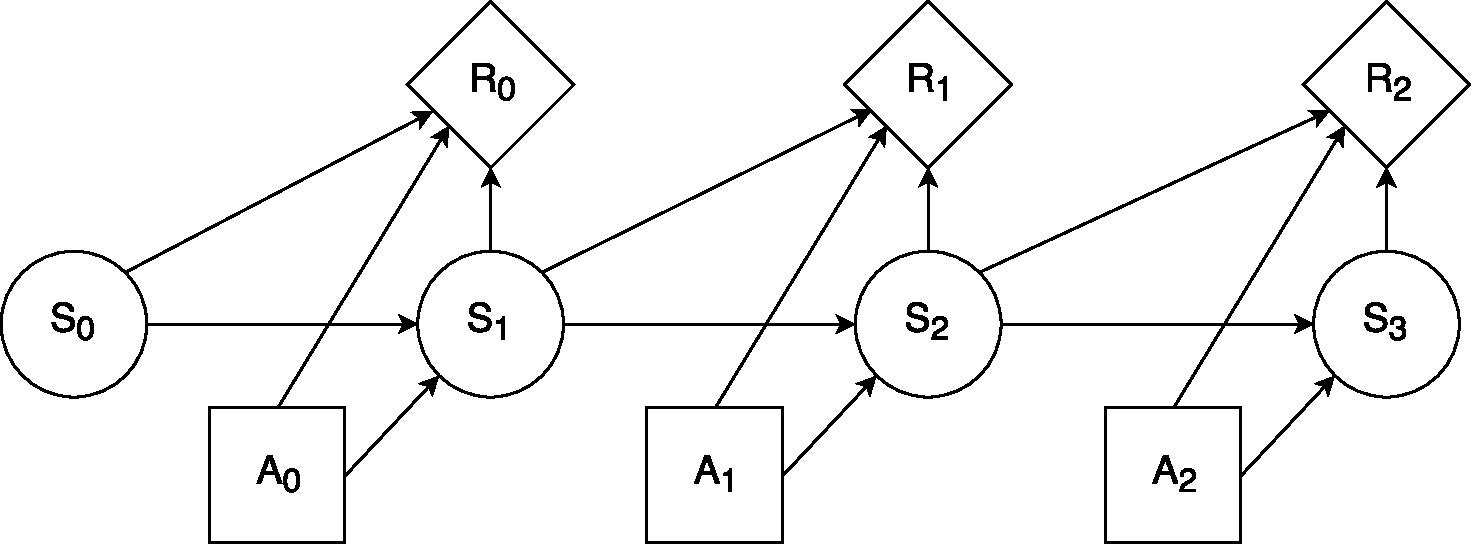
\includegraphics[width=10cm]{Figures/MDP}
\caption{Sample schematic of an MDP.}
\label{fig:MDP}
\end{figure}


\subsection{Q-learning}
Now that we contextualised reinforcement learning environments as Markov Decision Processes, we can introduce the final objective of reinforcement learning tasks: finding a function $\Pi:S\mapsto A$ called \textbf{policy}, that maps the appropriate action $a\in A$ given the current state $s\in S$, as to maximise our agent's final reward.

In particular, we will now present Q-learning, an algorithm that yields such optimal policy given an MDP.

Q-learning lets us learn the \emph{quality}, or expected utility, for each state-action combination. That is, for each state, let's estimate all the expected rewards we obtain by taking each possible action at that particular state.

More formally, we estimate a function $Q: S \times A \to \mathbb{R}$. We can model $Q$ as a mapping table (initialised with some uniform values), whose value we update at each time step of our simulations.

Here's how we update our Q-table at each time step $t$:
  \[Q(s_{t},a_{t}) = \underbrace{Q(s_t,a_t)}_{\rm old~value} +
  \underbrace{\alpha}_{\rm learning~rate} \times \left[
    \overbrace{\underbrace{r_{t+1}}_{\rm reward} + \underbrace{\gamma}_{\rm
        discount~factor} \underbrace{\max_{a}Q(s_{t+1}, a)}_{\rm
        estimate~of~optimal~future~value}}^{\rm learned~value} -
    \underbrace{Q(s_t,a_t)}_{\rm old~value} \right] \]
    
where:
\begin{itemize}
	\item $\alpha\in[0,1]$ is the \emph{learning rate}, a coefficient that regulates how much the newly learned values will contribute in the update
	\item $\gamma\in[0,1]$ is the \emph{discount factor}, a coefficient that controls the weight of future rewards. Values closer to 0 will make our agent "short-sighted", considering only the immediate rewards.
\end{itemize}

What is our optimal policy when we do Q-learning then? After training, it is simply that function $\pi: S \to A$ that, for each state, returns the action with maximum expected utility in our Q-table.

\subsection{Exploration/Exploitation tradeoff}
An important theme in reinforcement learning, and that we heavily focus our attention on in our project is the idea of the tradeoff between Exploration and Exploidation.

\subsection{Deep Reinforcement Learning}
\subsubsection{DQGAN}
\subsection{Problems with reinforcement learning techniques}
\subsection{Actor critic}

%----------------------------------------------------------------------------------------

\section{Generative Adversarial Networks}
\subsection{Architecture of GANs}
\subsection{Successes}
\subsubsection{DCGAN}
\subsection{Conditional GANs}

%----------------------------------------------------------------------------------------

\section{Existing related work}
\subsection{Generative Adversarial Imitation Learning}

%---------------------------------------------------------------------------------------- 
% Chapter 3

\chapter{Environment} % Main chapter title

\label{Chapter3} % For referencing the chapter elsewhere, use \ref{Chapter3} 

%----------------------------------------------------------------------------------------

In this chapter we report the process that went into choosing the environments that we will be using in the project's simulations, and from which we will be basing our simulations.

There are many choices of environments and tasks that are publicly available. Some of these we will be introducing in this chapter.

What makes this step non-trivial and deserving of its own chapter is that different reinforcement learning techniques are more suitable to different categories of tasks. Similarly, different machine learning and deep learning techniques are more or less efficient when applied to different tasks.

In a research effort that is heavily dependent on building reinforcement learning and deep learning models, the choice of environment is a critical one.

Furthermore, we also need to achieve this without losing focus on the main motivations for the whole project (Chapter~\ref{Chapter1}): \textit{optimising reinforcement learning algorithms by adding transferability of pre-trained models on unseen maps or configurations of a task}.

This last point implies that a substantial part of the computational work in the project will be about training hundreds of thousands of reinforcement learning models to build a dataset over a distribution of different maps (we present this in Chapter~\ref{Chapter4}). This is an important point: in the many experiments we ran, this turned out to be the biggest bottleneck, and required plans to distribute computations across multiple machines to make the computational time feasible in the timespan allocated to the project.

With these points in mind and given the experimental nature of the work, we conclude that a bottom-up approach in complexity is preferable. Given successful results with "easier" tasks, we can scale up in complexity and hopefully formalise and generalise our approach to more tasks (Chapter~\ref{Chapter7}).

Easier tasks will enable us to explore different reinforcement learning approaches that we introduced in Subsection~\ref{RL} with the guarantee that they will give satisfiable results. We can use these results as a foundation of the further steps (specifically Generative Adversarial Networks training in Chapter~\ref{Chapter5}).

Before introducing candidate environments, let us define what is meant by an "easy" reinforcement learning task. What we are looking for is ideally a task with a discrete and relatively small set of observable states and actions. Why does this condition make the task easier?

Imagine building a decision tree (such as the one shown in figure~\ref{fig:RLTree} with all possible states-action transitions, until we either: 1) reach a goal state, or 2) reach an arbitrarily maximum iteration time step $t = \eta$ or depth of the tree (to prevent infinite iterations). Also assume we were building this tree in a bruteforce manner (worst-case scenario of reinforcement learning resolutions), such that we need to build all possible paths or trajectory that the agent will need to take. Therefore, we would need to visit each node of the tree, until we arrive at the leaves. At the leaves, we can find the achieved reward for the agent given the path it has taken to get there. 

The breath and depth of the state-action tree will increase as we increase the possible set of states we would need to traverse, adding up to the space and time complexity of our solution, which is exponential in $\#S$ and $\#A$ for both space and time ($\#S$ indicates the cardinality of a set S).

With that said, there is a solid line between our ideal environment and a trivial one that could be solved without the aid of reinforcement learning techniques.

Let's explore some candidate environments next.
\begin{figure}
\centering
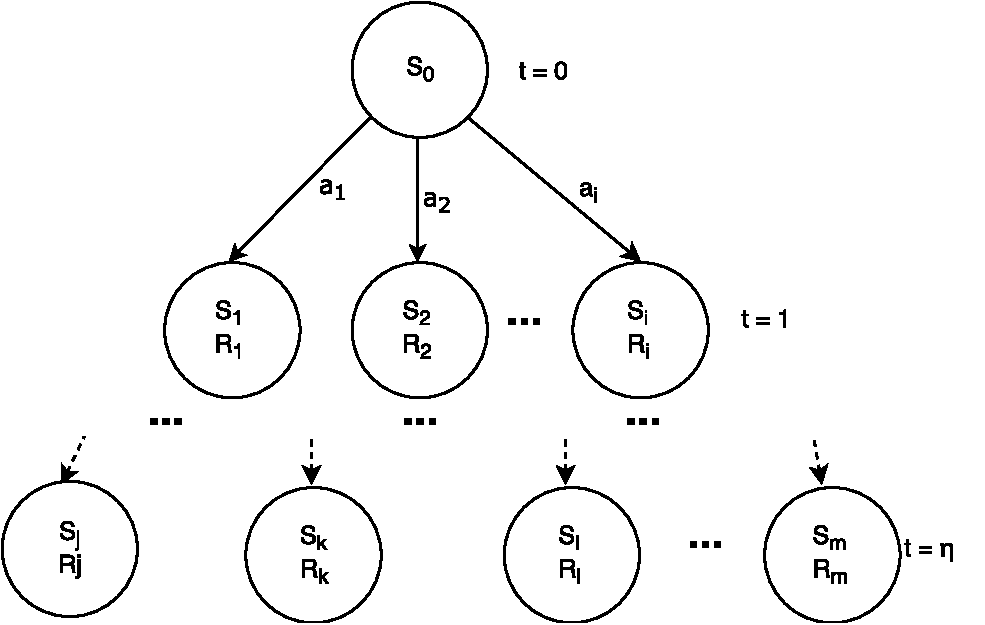
\includegraphics[width=7cm]{Figures/RLTree}
\caption{Sample state-action tree}
\label{fig:RLTree}
\end{figure}

\section{OpenAI Gym}
\label{openaigym}
OpenAI Gym \parencite{1606.01540} provides a toolkit that aids in the process of building reinforcement learning systems and evaluating algorithms to solve such tasks.

OpenAI Gym provides an environment interface \code{Env}. The interface abstracts the following operations on an environment:

\begin{itemize}
	\item \code{step(action)} -- Simulates one time step by executing the provided action. This returns \code{observation} (the new current state), the \code{reward} for taking such action, a flag \code{done} indicating whether the system has reached a final state, and \code{info} providing additional information dependent on the environment.
	\item \code{reset()} -- Resets the environment, i.e. the initial state is restored
	\item \code{render()} -- Renders the environment in human-readable format.
\end{itemize}

Now, we could either build implementations for such interface (if we were to implement our own environment's logic), or use the provided implementations for several environments in the OpenAI Gym library, which includes board games, algorithm-based or physics-based environments, Atari games, etc.

\subsection{Motivation}
In this project we will mostly deal with environments provided in the OpenAI Gym. There are several reasons for such decision:

\begin{itemize}
	\item It abstracts the need to implement the logic of a separate environment. Implementing our own environment adds a point of failure to our whole (quite experimental) work, as well as imposing a bigger time constraint to the one we already have;
	\item OpenAI Gym has become a standard academic tool for reinforcement learning researchers, therefore many papers and articles build on top of this framework;
	\item Environment implementations in the OpenAI Gym library are constantly expanding and being revised by an active community, also thanks to the support of the overarching organisation (OpenAI);
	\item The core implementation of the \code{gym} module \parencite{gymgymat12:online} allows for straightforward extensions on existing environments, which, as we will see in subsection~\ref{ExtendedBaseline}, will be critical in this project;
	\item While sadly not applicable anymore, OpenAI Gym used to provide and support an online platform for developers to compare the performance of different reinforcement learning algorithms for each task. This was in a form of a leaderboard, measuring the performances, as well as providing the implementation and data of winning techniques. Such data could have been used directly as input to our Generative Adversarial Networks.
\end{itemize}

\subsection{Algorithmic environments}
\subsection{MuJoCo and physics environments}
\subsection{Other environments}

%----------------------------------------------------------------------------------------

\section{Baseline: \code{FrozenLake-v0}}
One of our baseline environments is \code{FrozenLake-v0} \parencite{OpenAIGy42:online}, one of the algorithmic environments provided in the OpenAI Gym. In this section we describe the task, motivation for choosing it as one of our baseline models, and some shortcomings that we faced in using this environment in our project's pipeline.
\subsection{Description of the task}
In \code{FrozenLake-v0} we control an agent in a grid world, more precisely the grid shown in figure~\ref{tab:FrozenLakev0}. The objective is to go from a starting tile (\code{S}) to a goal state (\code{G}), by moving in four possible directions from a tile: \code{up}, \code{down}, \code{left} and \code{right}.

What differentiates this from a trivial path-finding or planning problem? A couple of things:
\begin{enumerate}
	\item there are both walkable and non-walkable tiles in the grid (these are respectively frozen tiles \code{F} and holes \code{H}), and
	\item tiles are "slippery", as in the agent could "slip" while navigating the grid world, meaning that the movement direction of the agent is uncertain and only partially depends on the direction we tell the agent to follow, i.e. the direction is non-deterministic.
\end{enumerate}

The reward in \code{FrozenLake-v0} is $1$ for reaching the goal state, and $0$ for being in any other state. The system stops executing when the agent falls into a hole, and the environment needs to be reset.

\begin{table}[]
\centering
\begin{tabular}{|c|c|c|c|}
\hline
\cellcolor[HTML]{68CBD0}\textbf{S} & F & F & F \\ \hline
F & \cellcolor[HTML]{CE6301}H & F & \cellcolor[HTML]{CE6301}H \\ \hline
F & F & F & \cellcolor[HTML]{CE6301}H \\ \hline
\cellcolor[HTML]{CE6301}H & F & F & \cellcolor[HTML]{32CB00}\textbf{G} \\ \hline
\end{tabular}
\caption{\code{FrozenLake-v0}'s default 4x4 configuration}
\label{tab:FrozenLakev0}
\end{table}

\subsection{Motivation and shortcomings}
\label{movationandshortcomings}
\code{FrozenLake-v0} is generally classified as a straightforward reinforcement learning task. An optimal solution could be found by creating a model of the environment, that is merely recording where frozen tiles are while exploring the grid world. This is a \emph{model-based} approach to reinforcement learning, and it is perhaps less interesting than learning by exploration, without being biased by the particular configurations of the map.

\emph{Model-free} algorithms, like Q-learning, need no accurate representation specific to the environment, and they are therefore more transferable to different configurations of the map or even to different tasks, which is the final objective of our project.

In fact, let's take the case of Q-learning applied to \code{FrozenLake-v0}: we do not need to have an explicit knowledge of the dynamics of each different tiles. We do not build a policy that explicitly favours movements towards frozen tiles or towards the goal. In fact, the agent does not have a model of what a frozen tile is, nor a model of the goal tile or a hole--it just learns by exploration that there it is rewarded when it gets to the goal state, and that is what it implicitly aims for.

This is the sort of behaviour that we can transfer to different tasks--again our ultimate objective.
\\\\
In its current OpenAI Gym implementation, \code{FrozenLake-v0} is a static map with the fixed configuration that is shown in figure~\ref{tab:FrozenLakev0}. There is currently no way to generate random configurations of the map, so next up, we will be extending this implementation to account for that.

\section{Extended baseline: Randomised Frozen Lake}
So we need to extend OpenAI Gym's implementation of \code{FrozenLake-v0} so that it can generate random configurations of the map.

Before we move on, let us contextualise this in the bigger picture as to not lose focus of what we are trying to achieve. Why do we need different configurations of the map, again? We want to train reinforcement learning models on different configurations so that we can have a distribution of policies over different maps which we can use as input to our GAN. After training our GAN, we will have a Generator network spawning new policies for unseen configurations without having to find it through (computationally expensive) reinforcement learning algorithms!
\\\\
Listing~\ref{lst:generate} shows how we implemented the algorithm to generate random maps. The critical line is line 4, which uses \code{numpy}'s \code{random.choice()} method that samples a matrix of a given size, given probabilities for each element (\code{'F'} and \code{'H'} tiles in our case).

So, we can pass in the desired size of the map. By default, it will generate 4x4 grids like the one in \code{FrozenLake-v0}, but we could generate maps of arbitrary size, which will result in higher task complexity. We explore these harder extensions in Chapter~\ref{Chapter7}. 

We can also pass it the probability that a tile will be a frozen one through the parameter \code{p}. The presence of fewer frozen tiles, and therefore of more holes, makes the goal harder to achieve for the agent.

\begin{minipage}{\linewidth}
\lstset{language=Python}
\lstset{frame=lines}
\lstset{caption={Algorithm to generate random configurations. Utility function \code{is\_valid()} of line 7 is shown in listing~\ref{lst:is_valid}}}
\lstset{label={lst:generate}}
\lstset{basicstyle=\footnotesize}
\begin{lstlisting}
def generate(size=4, p=0.8):
    valid_map = False
    while not valid_map:
        config = np.random.choice(['F','H'], (size, size), p=[p, 1-p])
        config[0][0] = 'S'   # set top left to be the starting tile
        config[-1][-1] = 'G' # set bottom right to be goal tile
        valid_map = is_valid(config)
        p *= 1.05            # increase probability of frozen tile
    return ["".join(x) for x in config]
\end{lstlisting}
\end{minipage}

Notice how the \code{generate()} function in listing~\ref{lst:generate} only returns valid maps, that is, maps that have at least one frozen path from start to goal. Surely, we could train models on environment configurations that are not solvable. Q-learning, for example, would just return a \code{Q} matrix with all Q-values equals to $0$, since the agent will never get to the goal tile and get its reward. If it is unclear why, refer to the Q-learning subsection~\ref{qlearning}.

Using such constraint on map validity, we can limit the number of models we need to train by a significant amount, therefore reducing training time.
\\\\
To check whether a map is solvable we use depth-first search from the start tile to the goal. If there is such path, then it is a valid map. Listing ~\ref{lst:is_valid} shows the algorithm:\\

\begin{minipage}{\linewidth}
\lstset{language=Python}
\lstset{frame=lines}
\lstset{caption={Depth-first search to check if a frozen lake map is valid}}
\lstset{label={lst:is_valid}}
\lstset{basicstyle=\footnotesize}
\begin{lstlisting}
def is_valid(arr, r=0, c=0):
    if arr[r][c] == 'G':
        return True

    tmp = arr[r][c]
    arr[r][c] = "#" # temporary mark with '#' to remember visited tiles
    
    if r+1 < size and arr[r+1][c] not in '#H': # go down
        if is_valid(arr, r+1, c) == True:
            arr[r][c] = tmp
            return True
    if c+1 < size and arr[r][c+1] not in '#H': # go right
        if is_valid(arr, r, c+1) == True:
            arr[r][c] = tmp
            return True
    if r-1 >= 0 and arr[r-1][c] not in '#H': # go up
        if is_valid(arr, r-1, c) == True:
            arr[r][c] = tmp
            return True
    if c-1 >= 0 and arr[r][c-1] not in '#H': # go left
        if is_valid(arr,r, c-1) == True:
            arr[r][c] = tmp
            return True
            
    arr[r][c] = tmp
    return False
\end{lstlisting}
\end{minipage}

So the \code{generate()} function returns a valid random frozen lake map represented as a list of strings. An example of an output is $["SFHH", "HFHH", "HFHH", "HFFG"]$. Each string in the list encodes a row configuration of the frozen lake.

What is left to do now, is to extend \code{FrozenLake-v0} so that we could pass in any map configuration, therefore exposing our randomly generate maps to the \code{gym} environment interface we described in earlier in section~\ref{openaigym}. Listing~\ref{lst:register} shows how to register a new environment by extending a pre-existing one.
\\\\
\begin{minipage}{\linewidth}
\lstset{language=Python}
\lstset{frame=lines}
\lstset{caption={Code to extend \code{FrozenLake-v0} with random maps.}}
\lstset{label={lst:register}}
\lstset{basicstyle=\footnotesize}
\begin{lstlisting}
random_map = generate(size=4, p=0.8)
register(
    id='RandomisedFrozenLake',
    entry_point='gym.envs.toy_text:FrozenLakeEnv',
    kwargs={'is_slippery': True, 'desc': random_map},
    max_episode_steps=100,
)
\end{lstlisting}
\end{minipage}

Now, to start doing simulations on our new environment we can just initialise it just like any other OpenAI Gym environment:

\begin{minipage}{\linewidth}
\lstset{language=Python}
\lstset{label={lst:register}}
\lstset{basicstyle=\footnotesize}
\begin{lstlisting}
env = gym.make('RandomisedFrozenLake')
\end{lstlisting}
\end{minipage}

We created a pull request to the OpenAI Gym's Github repository integrating this feature supporting random maps for \code{FrozenLake-v0}, so that developers and researchers could make use of these functionalities \parencite{Addabili86:online}.

\label{ExtendedBaseline}
% Chapter 4

\chapter{Dataset creation}
\label{Chapter4}

In Chapter~\ref{Chapter3} we finalised our OpenAI environment choice and have a systematic way to generate different configurations of our environments.

The next step is to build up our dataset by solving as many of these configurations as possible with the use of reinforcement learning algorithms.

We justified in previous sections (specifically section~\ref{qlearning} and section~\ref{movationandshortcomings}) how using \emph{model-free} reinforcement learning algorithms will put us in the right direction to achieve the project's goals highlighted in section~\ref{motivation}: improve the transferability of pre-trained models to different configurations, environments, and tasks.

One choice that is left to make before we move on to train models using our randomised environments is what reinforcement learning algorithm we should use.

%----------------------------------------------------------------------------------------

\section{Q-learning on \code{RandomisedFrozenLake}}
We have presented Q-learning in section~\ref{qlearning} as a method that generates a policy by building up a table $Q$ of values corresponding to the expected utility of taking each action at each observable state.

This table $Q$ is represented as a 2D-matrix of size (\code{env.observation\_space.n}, \code{env.action\_space.n}), which in the case of \code{RandomisedFrozenLake} is just a (16x4) matrix.

This is good news. Having a policy that is encoded as a 2-dimensional data structure makes it an obvious input to our Generative Adversarial Network later on in the next chapter. In fact, as we presented in section~\ref{successes}, GANs have proven successful in image synthesis applications, where inputs were images, that is 2D matrices.

The choice of Q-learning as our reinforcement learning technique therefore becomes preferable. Other model-free algorithms like policy search may not have a clear 2D representation in the way the trained parameter set $\theta$ is encoded.

%----------------------------------------------------------------------------------------

\section{Experiment set up}
Before we proceed, we need to be able to record some details about the process of training our data. If our ultimate objective is to benchmark performance of traditional reinforcement learning agains our proposed approach, we need to record running time of our training, and see if that improves at the end. 

Let's encapsulate training of a configuration in an \code{Experiment} class, whose code is shown in listing~\ref{lst:experiment}. An \code{Experiment} is initialised with an OpenAI Gym environment, which in our case is an instance of a \code{RandomisedFrozenLake}, and an integer value \code{num\_episodes}, indicating the number of independent simulations the Q-learning algorithm will be doing. By calling \code{Experiment}'s \code{run()} instance method, we actually start training the model, with $Q$ being updated at each iteration.

The instance variable \code{score} could be used as an evaluation criteria of the effectiveness of our training. It records the average reward the agent achieves for each episode during training.

\code{Experiment} also has a utility method called \code{dumps()} that serialises all this data and allows us to save it on disk.
\\\\
\begin{minipage}{\linewidth}
\lstset{language=Python}
\lstset{frame=lines}
\lstset{caption={\code{Experiment} wrapper class to train one instance of \code{RandomisedFrozenLake}}}
\lstset{label={lst:experiment}}
\lstset{basicstyle=\footnotesize}
\begin{lstlisting}
class Experiment(object):
    def __init__(self, env, num_episodes=10000):
        self.env = env
        self.Q = np.zeros([self.env.observation_space.n, self.env.action_space.n])
        self.num_episodes = num_episodes
        self.score = None
        self.valid_score = None
        self.start = None
        self.end = None
            
    def run(self):
        self.start = datetime.now()
        # ------------------------------------------------------------
        # Run Q-learning algorithm, saving the rewards of each episode
        # ...
        # ...
        # ------------------------------------------------------------
        self.end = datetime.now()
        self.score = sum(rewards)/self.num_episodes
        
    def dumps(self):
        return dumps({'Q': self.Q, 'start': self.start, 'end': self.end, 'score': self.score, 'num_episodes': self.num_episodes})
\end{lstlisting}
\end{minipage}

It's critical to be able to evaluate the quality of the Q-table after training. To do so we just use the optimal policy (that is the policy that picks the action that has the maximum expected utility according to the Q-table) and run if for a certain number of episodes. A validation score could be then defined by the average reward achieved at each episode. Listing \ref{lst:validate_experiment} shows the code to achieve that.

\begin{minipage}{\linewidth}
\lstset{language=Python}
\lstset{frame=lines}
\lstset{caption={Code to validate a trained Q-table}}
\lstset{label={lst:validate_experiment}}
\lstset{basicstyle=\footnotesize}
\begin{lstlisting}
def validate(self):
	rewards = 0
    for i in tqdm(range(num_episodes)):
        while j < 200: # Limit to 200 time steps
            j+=1
            # Choose an action by pick best action from Q-table
            a = np.argmax(Q[s,:])
            
            # Get new state and reward from environment
            s1,r,d,_ = env.step(a)
            rewards += r
            s = s1
            if d == True:
                break
     self.valid_score = rewards / num_episodes
\end{lstlisting}
\end{minipage}

%----------------------------------------------------------------------------------------

\section{Distributing Q-learning with MapReduce}
Now that we formalised our experiment setup, we can run Q-learning on each of the map configurations of our \code{RandomisedFrozenLake}. For the 4x4 grid there are 3,827 possible valid map configurations. It takes an average of 15 seconds to train each Q-learning table on a 2.5 GHz Intel Core i7 processor. On a single machine, it would take around 16 CPU hours to run the whole set of experiments.

To make this step of our pipeline faster and scalable to more data, we decide to set up a distributed processing on a cluster with multiple machines. More precisely, we set up a MapReduce framework \parencite{Dean:2004:MSD:1251254.1251264} implementation running on an Hadoop cluster \parencite{shvachko2010hadoop} of 25 machines.

A MapReduce program is composed of a Map procedure that takes in some (large) input and performs a particular operation whose output is then fed into another Reduce procedure, which outputs the final result. The power of MapReduce is that the framework orchestrates the processing of these procedures by marshalling the distributed servers, running the various tasks in parallel, managing all communications and data transfers between the various parts of the system, and providing for redundancy and fault tolerance.

Figure~\ref{fig:MapReduce} shows the distributed architecture to train multiple Q-learning instances. The input to the system is a list of strings, each representing the map configuration of a \code{RandomisedFrozenLake}, e.g. $"SFHHHFHHHFHHHFFG"$. These inputs are fed into Mapper programs running on different machines. The mapper's task is to initialise the experiment and run Q-learning on the environment. It outputs a key-value pair, where the key is the string that uniquely identifies a map configuration, and the output is the \code{Experiment} object that encapsulates the already trained Q-table. We have yet to assign a validation score to this table we trained, and that's the job of the reducer.

Each experiment's result is then written to an output file by the reducer. Each line will be again a key-value pair, with the map configuration string as key and the \code{Experiment} result dumped in string format. In the following sections, we can just parse and load these results to conduct our further analysis.

While this particular architecture does not make full use of the power of MapReduce (combining, partitioning and sorting), it is an optimal and convenient pipeline to distribute our computations across a cluster of machines, thereby drastically reducing the training time of the whole experiment set.
\begin{figure}
\centering
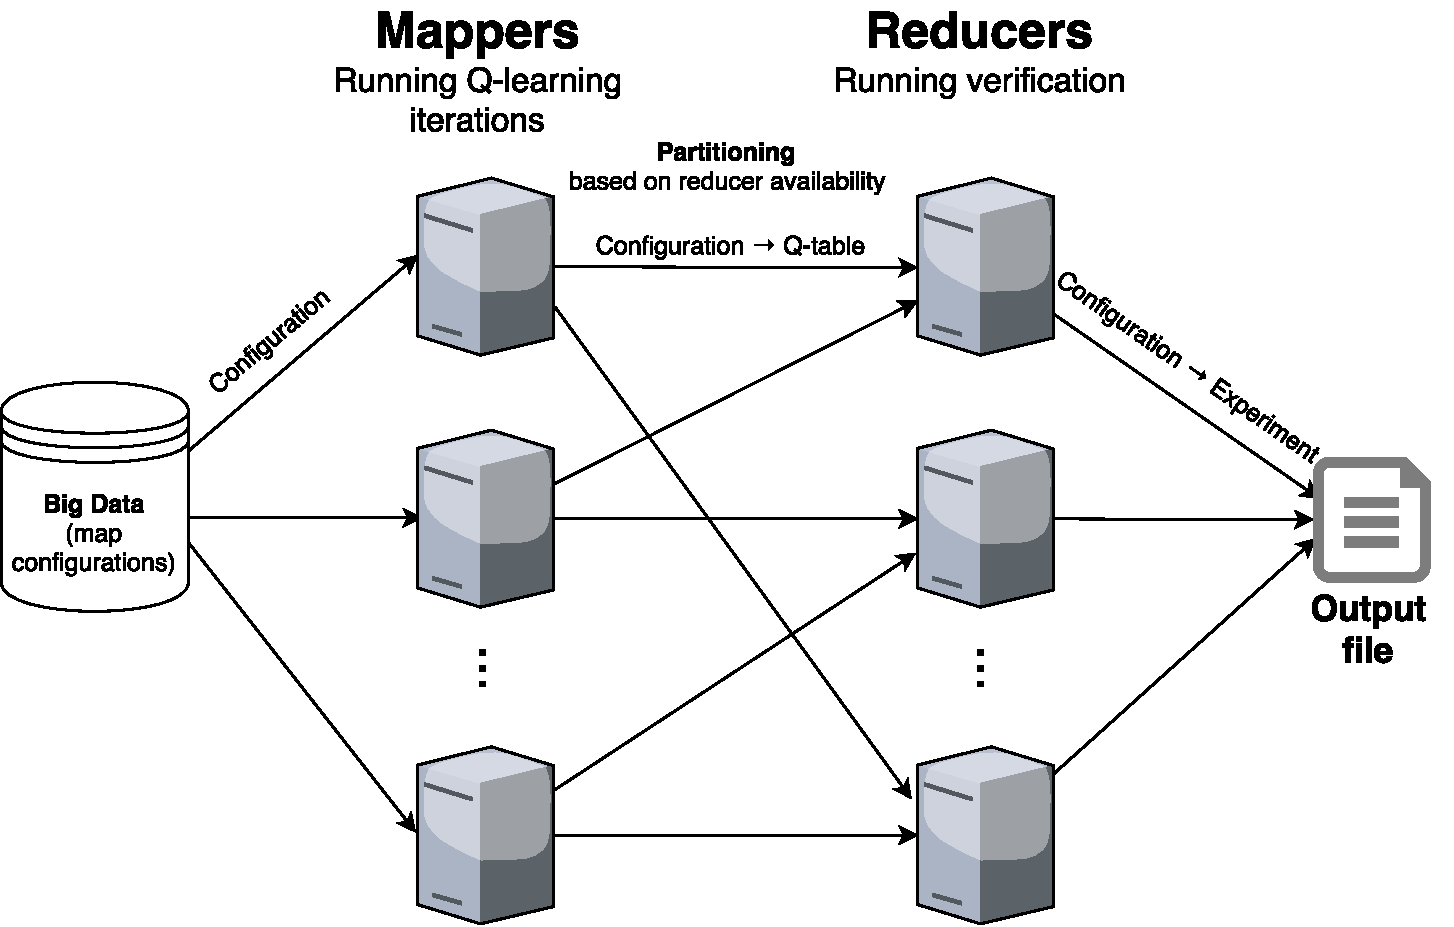
\includegraphics[width=10cm]{Figures/MapReduce}
\caption{Schematic of distributed Q-learning with validation on MapReduce}
\label{fig:MapReduce}
\end{figure}

\section{Analysis of results}
\label{sec:analysisresults}
In this section we report some statistics on the data we just trained. This analysis will be useful when we perform our final benchmarking.

Figure~\ref{fig:Qvalues} shows the average intensity values of the Q-tables in the training subset.

We notice that the utility values in the second and third columns are, in most cases, the highest values at each row. We interpret this as our models favouring, on average, the action of going south (second column) and east (third column) over going west or north.

Indeed, according to the reward system that we described in section~\ref{sec:adjrewardsys}, our trained models will try and reach the goal state with as few actions as possible. This validates why on average, the best actions to make at each state will be going south or going east.
% TODO: Plot rewards plot with std
% TODO: Define acceptable line and when it is achieved

STILL NEED TO FINISH THIS ANALYSIS
\begin{figure}
\centering
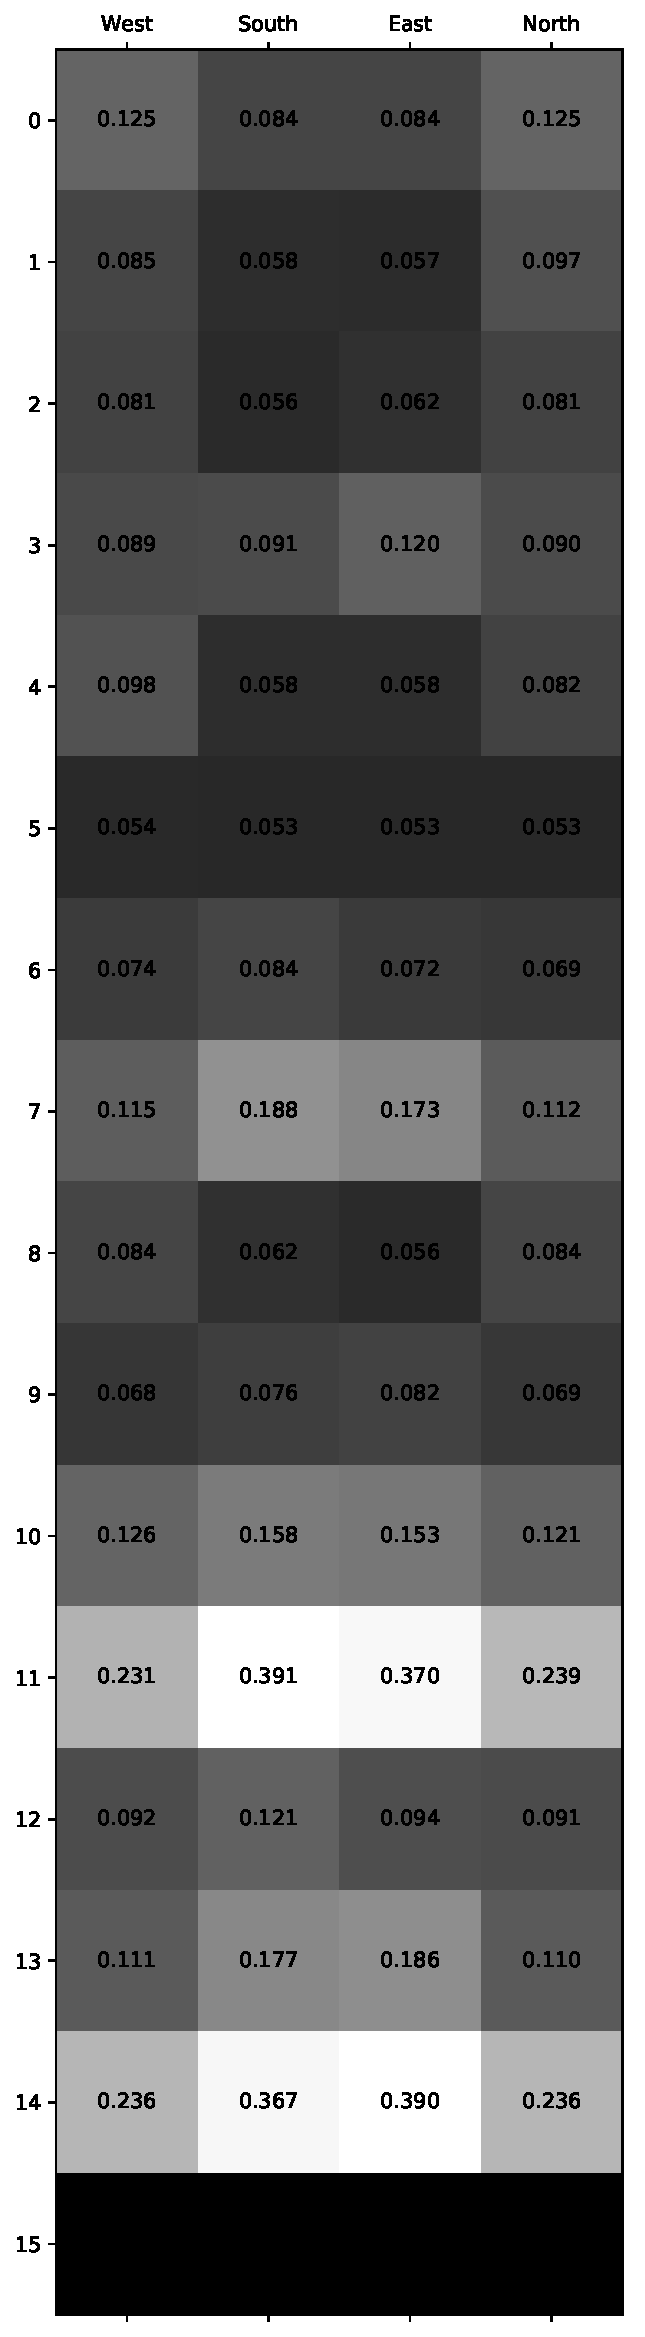
\includegraphics[width=3cm]{Figures/Qtable_mean}
\caption{Average intensity values of the Q-tables in the training subset}
\label{fig:Qvalues}
\end{figure}

\section{Transferable knowledge}
\label{sec:transferableknowledge}
Before proceeding, we need to start a discussion on the type of knowledge that we wish or we expect to be transferred. Having transferred knowledge is what will allow us to speed up training time on unseen tasks.

By using Q-learning to train policies on \code{RandomisedFrozenLake}, we effectively train agents to go from the top-left corner to the bottom-right corner.
In section~\ref{sec:adjrewardsys} we adjusted the reward system so that we reward the agent more if it reaches the goal state in fewer time steps. We implicitly favour actions that go south or east. We have just seen in our results analysis how on average the agent is indeed inclined towards the south-east direction.

In this lays our expectation for transferred knowledge: we hope that this bias towards south-east directions in our distribution of training policies is captured by our Generative Adversarial Network.

If that is the case, we can therefore use this captured knowledge when we train new policies on unseen tasks in the test set of map configurations.

In fact, we expect the training process on new maps to be faster given the knowledge that in order to reach goal state, we should give priority to the south-east direction.

As an intuition, imagine there are two people in a labyrinth, looking for a treasure. The first person knows that they will likely eventually find the treasure if they keep going south-east. The other does not. We expect the first one to reach the treasure much faster. The concept of "going south-east" is the knowledge that we hope to transfer in this task domain.

\section{Task generalisation}
\label{sec:taskgeneralisation}
We explained how we hope to capture transferrable knowledge that is generalisable across similar tasks. We do so by training a GAN using the policy distribution in our training set of policies, and we show this process in the next chapter (Chapter~\ref{Chapter5}).

Before we do that, we ought to talk about how this pipeline generalises on different reinforcement learning task domains. In our work we focused on the Frozen Lake environments, but the ultimate goal of our work is to develop a data pipeline that generalises to most reinforcement learning task domains.

If we hope to transfer knowledge within a domain, one key requirement is that there needs to be transferrable knowledge across these tasks. In our main experiment, we decoded this as being the action of "going south-east". However, with many and more complex domains with a larger action space and observation space, it may not be as trivial to identify such knowledge.

In our work, one of the reasons we chose Frozen Lake environments is that it is straightforward enough to verify that our agents are leveraging and benefitting from previous knowledge.

But in many other applications, we do not expect to be able to even decode the transferred knowledge in words, as we do when we say "going south-east". We will leave that up to the deep neural networks and their inherent statistical foundations to model such behaviour given the distribution we pass it.

By developing our pipeline for transferring knowledge, we provide a generalisable tool that people can use on their own task domains.

%---------------------------------------------------------------------------------------- 
% Chapter 1

\chapter{Adversarial Networks Training} % Main chapter title

\label{Chapter5} % For referencing the chapter elsewhere, use \ref{Chapter1} 

%----------------------------------------------------------------------------------------



% Chapter 6

\chapter{Generative Adversarial Transfer Learning} % Main chapter title
\label{Chapter6}
At this point of our Data Pipeline, we have two trained deep neural networks: the Generator \code{G} and the Discriminator \code{D}. It is once again important to contextualise this work in the Data Pipeline presented in section~\ref{sec:datapipeline} and as we showed it in figure~\ref{fig:pipeline}.

\code{G} is able to generate Q-tables, which we can effectively consider our optimal policies that solve a set of similar tasks. \code{D} returns an indication of on the "realness" or quality of a Q-table.
Both \code{G} and \code{D} hopefully capture the data distribution of the training data, which were just a subset of the Q-tables we generated in Chapter~\ref{Chapter4}.

Next up in our work is to develop and propose different reinforcement learning algorithms that can leverage the knowledge that we captured through the Generative Adversarial Network. We aim to transfer such knowledge to the tasks in the test set. We hope to achieve better rewards as well as lower training times than the policies we trained with vanilla Q-learning.

The algorithms that we propose in this Chapter mostly build on the Q-learning procedure that we presented back in section~\ref{qlearning}. In the techniques that we propose, we integrate Q-learning with the Generator \code{G} and Discriminator \code{D} neural networks in different ways.

In the context of our discussion on task generalisation that we already started in section~\ref{sec:taskgeneralisation}, we also need to discuss how these techniques generalise to other reinforcement learning task domains. 

We empirically test all these techniques on our \code{RandomisedFrozenLake} environment setup, and therefore we get an indication on the successes and failures of such techniques with a bias on this environment. We report the results of each technique in the following chapter (Chapter~\ref{Chapter7} - Benchmarking).

Given this disclaimer, we nevertheless endeavour to provide a data pipeline for transfer learning using GANs that generalises as much as possible to any reinforcement learning task.

Because of this, some of the techniques we propose here have not necessarily been successful with our environment setup, but can, within reasonable expectations, be in other task domains with different transferred knowledge, environment dynamics, and data distributions of policies.

As it is common in reinforcement learning and deep learning applications, empirical exploration of different techniques is the most effective way to verify which is a best fit in the given problem.

%----------------------------------------------------------------------------------------
\section{Using the trained Discriminator}
The Discriminator network \code{D} takes in as an input a Q-table, and outputs a single scalar in $[0,1]$ representing the predicted probability that the inputted Q-table is a genuine one.

One way to leverage this to achieve our goal is by asking the following question:\\

\begin{addmargin}[2.5em]{2.5em}
"How should we update the values of the Q-table that we inputted to \code{D}, so that if we input the updated Q-table, the score that the Discriminator returns is higher (i.e. the Q-table becomes more genuine)?"\\
\end{addmargin}

This in fact turns out to be the same fundamental question of any gradient-based optimisation technique in machine learning. When doing vanilla gradient descent, for example, we ask ourselves a similar question: "how should we update our model's parameter set so that we minimise the loss function?", the answer to which is "by moving in the opposite direction of the loss function's gradient with respect to our parameter".

This gives us a way to find a Q-table update. The loss function in our case is how far we are from having the discriminator label the Q-table as being real, that is how far is the predicted output from a label of one: $1 - y_{predicted}$.

So what we need to calculate is the discriminator loss's gradient with respect to the Q-table, which we call $\nabla D(Q_{t})$.

Recall the algorithm for Q-learning. The way we can use $\nabla D(Q_{t})$ is by combining the vanilla Q-learning update step of equation~\ref{eq:QlearningUpdate} to an update with the gradient step.

\begin{algorithm}[H]
\caption{Q-learning with gradient update}
\begin{algorithmic}[1]
\Require
 	\State $S$ is a set of states
 	\State $A$ is a set of actions
 	\State $\gamma$ the discount reward factor
 	\State $\alpha$ is the learning rate
 	\State $n$ is number of episodes to run Q-learning
 	\State $\epsilon$, probability to take random action, rather than follow policy
\Procedure{Q-Learning} {}
\\Initialize $Q(s,a)$ will all 0 utility values.
\For{each episode $e_i$ with $i=0...n$}
\\ \qquad Initialize $s$
\For{each step of episode}
\\ \qquad \qquad Choose $a_t$ from $s_t$ using policy derived from $Q$ with $\epsilon$-Greedy
\\ \qquad \qquad Take action $a_t$, observe reward $r$ and $s_{t+1}$
\\ \qquad \qquad Update Q-table using $\nabla D(Q_{t})$
\EndFor
\EndFor
\EndProcedure
\end{algorithmic}
\end{algorithm}

\subsection{Baselines approach: Q-learning and L2 regulariser}
\label{ssec:QlearningBaseline}

This is the basic update step of vanilla Q-learning.

\begin{equation} \label{eq:QlearningUpdate}
\begin{aligned}
  Q(s_{t},a_{t}) ={} & \underbrace{Q(s_t,a_t)}_{\rm old~value} +
  \underbrace{\alpha}_{\rm learning~rate} \times \\
   & \times \left[
    \overbrace{\underbrace{r_{t+1}}_{\rm reward} + \underbrace{\gamma}_{\rm
        discount~factor} \underbrace{\max_{a}Q(s_{t+1}, a)}_{\rm
        estimate~of~optimal~future~value}}^{\rm learned~value} -
    \underbrace{Q(s_t,a_t)}_{\rm old~value} \right]
\end{aligned}
\end{equation}

Another baseline model that we can consider is the one that transfers knowledge through L2 regularisation, by pushing the Q-table towards the average of the tasks in the train set. In figure~\ref{fig:Qvalues} we displayed such mean values of the train set. With this regulariser we try to take a step towards this average.

\subsection{Approach 1: Update whole Q-table towards $\nabla D(Q_{t})$}
\label{ssec:QlearningGANWhole}
In this approach we update whole Q-table in the direction of the gradient. We precede this with a vanilla Q-learning update step.

\begin{equation}
Q_{t+1} = Q_{t}-\underbrace{\beta}_{\rm discriminator~learning~rate} \times \underbrace{\nabla D(Q_{t})}_{\rm gradient~of~D~at~Q_{t}}
\end{equation}

\subsection{Approach 2: Update state/action value pair towards $\nabla D(Q_{t})$}
\label{ssec:QlearningGANPair}
This approach is similar to the one before, but just like Q-learning, we only update the state/action pair of the step the agent just took in the environment. This approach combines Q-learning's update approach with our gradient-based update.

\begin{equation}
\begin{aligned}
  Q(s_{t},a_{t}) ={} &\underbrace{Q(s_t,a_t)}_{\rm old~value} + \\
  & + \underbrace{\alpha}_{\rm learning~rate} \times \left[
    \overbrace{\underbrace{r_{t+1}}_{\rm reward} + \underbrace{\gamma}_{\rm
        discount~factor} \underbrace{\max_{a}Q(s_{t+1}, a)}_{\rm
        estimate~of~optimal~future~value}}^{\rm learned~value} - \underbrace{Q(s_t,a_t)}_{\rm old~value} \right] + \\
   & - \underbrace{\beta}_{\rm discriminator~learning~rate} \times \underbrace{\nabla D(Q)(s_{t}, a_{t})}_{\rm gradient~of~D~at~Q_{t}}
\end{aligned}
\end{equation}

\subsection{Approach 3: Update state/action row towards $\nabla D(Q_{t})$}
\label{ssec:QlearningGANRow}
Similar to the approaches above, but updates the whole row of actions for the state the agent is in.

\begin{equation}
\begin{aligned}
  \forall a \in A: \\
  Q(s_{t},a) ={} &\underbrace{Q(s_t,a)}_{\rm old~value} + \\
  & + \underbrace{\alpha}_{\rm learning~rate} \times \left[
    \overbrace{\underbrace{r_{t+1}}_{\rm reward} + \underbrace{\gamma}_{\rm
        discount~factor} \underbrace{\max_{a}Q(s_{t+1}, a)}_{\rm
        estimate~of~optimal~future~value}}^{\rm learned~value} - \underbrace{Q(s_t,a)}_{\rm old~value} \right] + \\
   & - \underbrace{\beta}_{\rm discriminator~learning~rate} \times \underbrace{\nabla D(Q)(s_{t}, a)}_{\rm gradient~of~D~at~Q_{t}}
\end{aligned}
\end{equation}

%   \[\frac{\sum_{i}^{test~set} valid\_score(Q_i) - valid\_score(Q_i')}{\#(test~set)}\]

%----------------------------------------------------------------------------------------

\section{Using the trained Generator}
We can categorise Q-learning and the approaches that we just presented as being "local search" in the space of possible policies that solve the task. That is, we search over possible Q-tables/policies by just applying local changes when we update the Q-table at each time step.

Another heuristic method for optimisation problems is global search, that is searching all possible solutions and choosing the one that maximises the achieved rewards.

\subsection{Approach 1: Global Search}
\label{ssec:globalsearch}
Global search is effectively a bruteforce method to obtain a policy that 
that solves a task. While this may seem like a non-optimal approach, if we already have a distribution of potential policies, global search may be the least computationally expensive approach.
In fact, we can try and sample a fixed number of Q-tables/policies from the Generator network, and check the rewards that each of these policies yields.

\subsection{Approach 2: Local/Global search hybrid}
\label{ssec:localglobalsearch}
The issue with global search, is that the solutions that we may find, while yielding good rewards, are not necessarily optimised for the specific task at hand. We could be achieving better overall rewards if we did some local search using the Q-table we found through global search.

To do that we can do our global search on a fixed number of sampled policies, and choose the best Q-table. 
Now, to do local search, we can choose any of approaches we introduced in the previous section, but instead of initialising the Q-table with 0 values, we initialise it as the Q-table we just found with global search.

\begin{algorithm}[H]
\caption{Global search and Q-learning with gradient update}
\begin{algorithmic}[1]
\Require
	\State $p$ number of policies to sample for global search
 	\State $S$ is a set of states
 	\State $A$ is a set of actions
 	\State $\gamma$ the discount reward factor
 	\State $\alpha$ is the learning rate
 	\State $n$ is number of episodes to run Q-learning
 	\State $\epsilon$, probability to take random action, rather than follow policy
\Procedure{Global Search} {}
\For{i in $i=0...p$}
\\ \qquad Sample Q-table from the Generator
\\ \qquad Evaluate the Q-table/policy
\EndFor
\\ Let $Q_{best}$ be the Q-table that yields the best policy
\EndProcedure
\Procedure{Q-Learning} {}
\\Initialize Q = $Q_{best}$
\For{each episode $e_i$ with $i=0...n$}
\\ \qquad Initialize $s$
\For{each step of episode}
\\ \qquad \qquad Choose $a_t$ from $s_t$ using policy derived from $Q$ with $\epsilon$-Greedy
\\ \qquad \qquad Take action $a_t$, observe reward $r$ and $s_{t+1}$
\\ \qquad \qquad Update Q-table using $\nabla D(Q_{t})$
\EndFor
\EndFor
\EndProcedure
\end{algorithmic}
\end{algorithm}


%----------------------------------------------------------------------------------------
% Chapter 7

\chapter{Benchmarking}
\label{Chapter7}

In this chapter we present several metrics that can be used to evaluate the performance of the transfer learning techniques that we presented in Chapter~\ref{Chapter6}.

We also report the results on our reinforcement learning domain following such metrics.

These metrics are important to critically evaluate and compare these techniques with baseline models.

% Baseline:
% Vanilla Q-learning
% Q-learning with L2 (towards zero) regularisation
% Q-learning with L2 (towards average of source tasks, conventional transfer learning) regularisation

% Metrics:
% Timestamp of acceptable reward
% AuC


\section{Metrics and baseline model}
\label{sec:metricsbaselinemodel}
One first step necessary to evaluate success in the resolution of reinforcement learning tasks is to plot the rewards over time, and verifying the asymptotic trend of the curve.

Usually these will converge to a certain value, which is indicative of the performance of the models that we trained. The approach that OpenAI takes in evaluating success of certain policy that has been trained is to set a fixed reward threshold above which the task is considered solved. For example, the vanilla \code{FrozenLake-v0} implementation with the fixed map configuration we showed in figure~\ref{tab:FrozenLakev0}, is considered "solved" if the policy achieves an average reward of 0.78 over 100 consecutive trials.

While our implementation of \code{RandomisedFrozenLake} directly builds on the \code{FrozenLake-v0} environment, using the same average reward threshold for our set up will not work. The reason being that the map configuration of \code{FrozenLake-v0} has a fixed degree of difficulty indicated by the number of holes in the map. The threshold of 0.78 directly has been set given this difficulty.
\code{RandomisedFrozenLake} environments have a varying amount of holes and, as a consequence, of difficulty. To set our threshold, we plot in figure~\ref{fig:QlearningBaselineBench} the average rewards achieved by the Q-tables in the test set while training with vanilla Q-learning. Each timestep corresponds to the average reward achieved with the 765 policies in the test set at the corresponding timestep. We also plot the standard deviations (dashed blue lines) of these rewards. Furthermore, to plot this curve we take the rolling window average of 20 timesteps to avoid wildly oscillating reward curves.

We notice right away that in fact we never even reach a value of 0.78 in our average rewards. That is because map configurations in the test set contain tasks that are on average harder (i.e. contain more holes) than \code{FrozenLake-v0}.

The test policies rewards asymptotically converge to 0.36, which may seem low compared to \code{FrozenLake-v0}'s 0.78, but it is once again taken as an average of all maps in the test set. That also justifies the wide standard deviations on the plot, as it virtually ranges the whole reward boundaries $(0,1)$.

Given this analysis, we set the average threshold reward value to 0.32 (grey dashed/dotted line), which vanilla Q-learning reaches after around 250,000 training timesteps.

\begin{figure}[H]
\centering
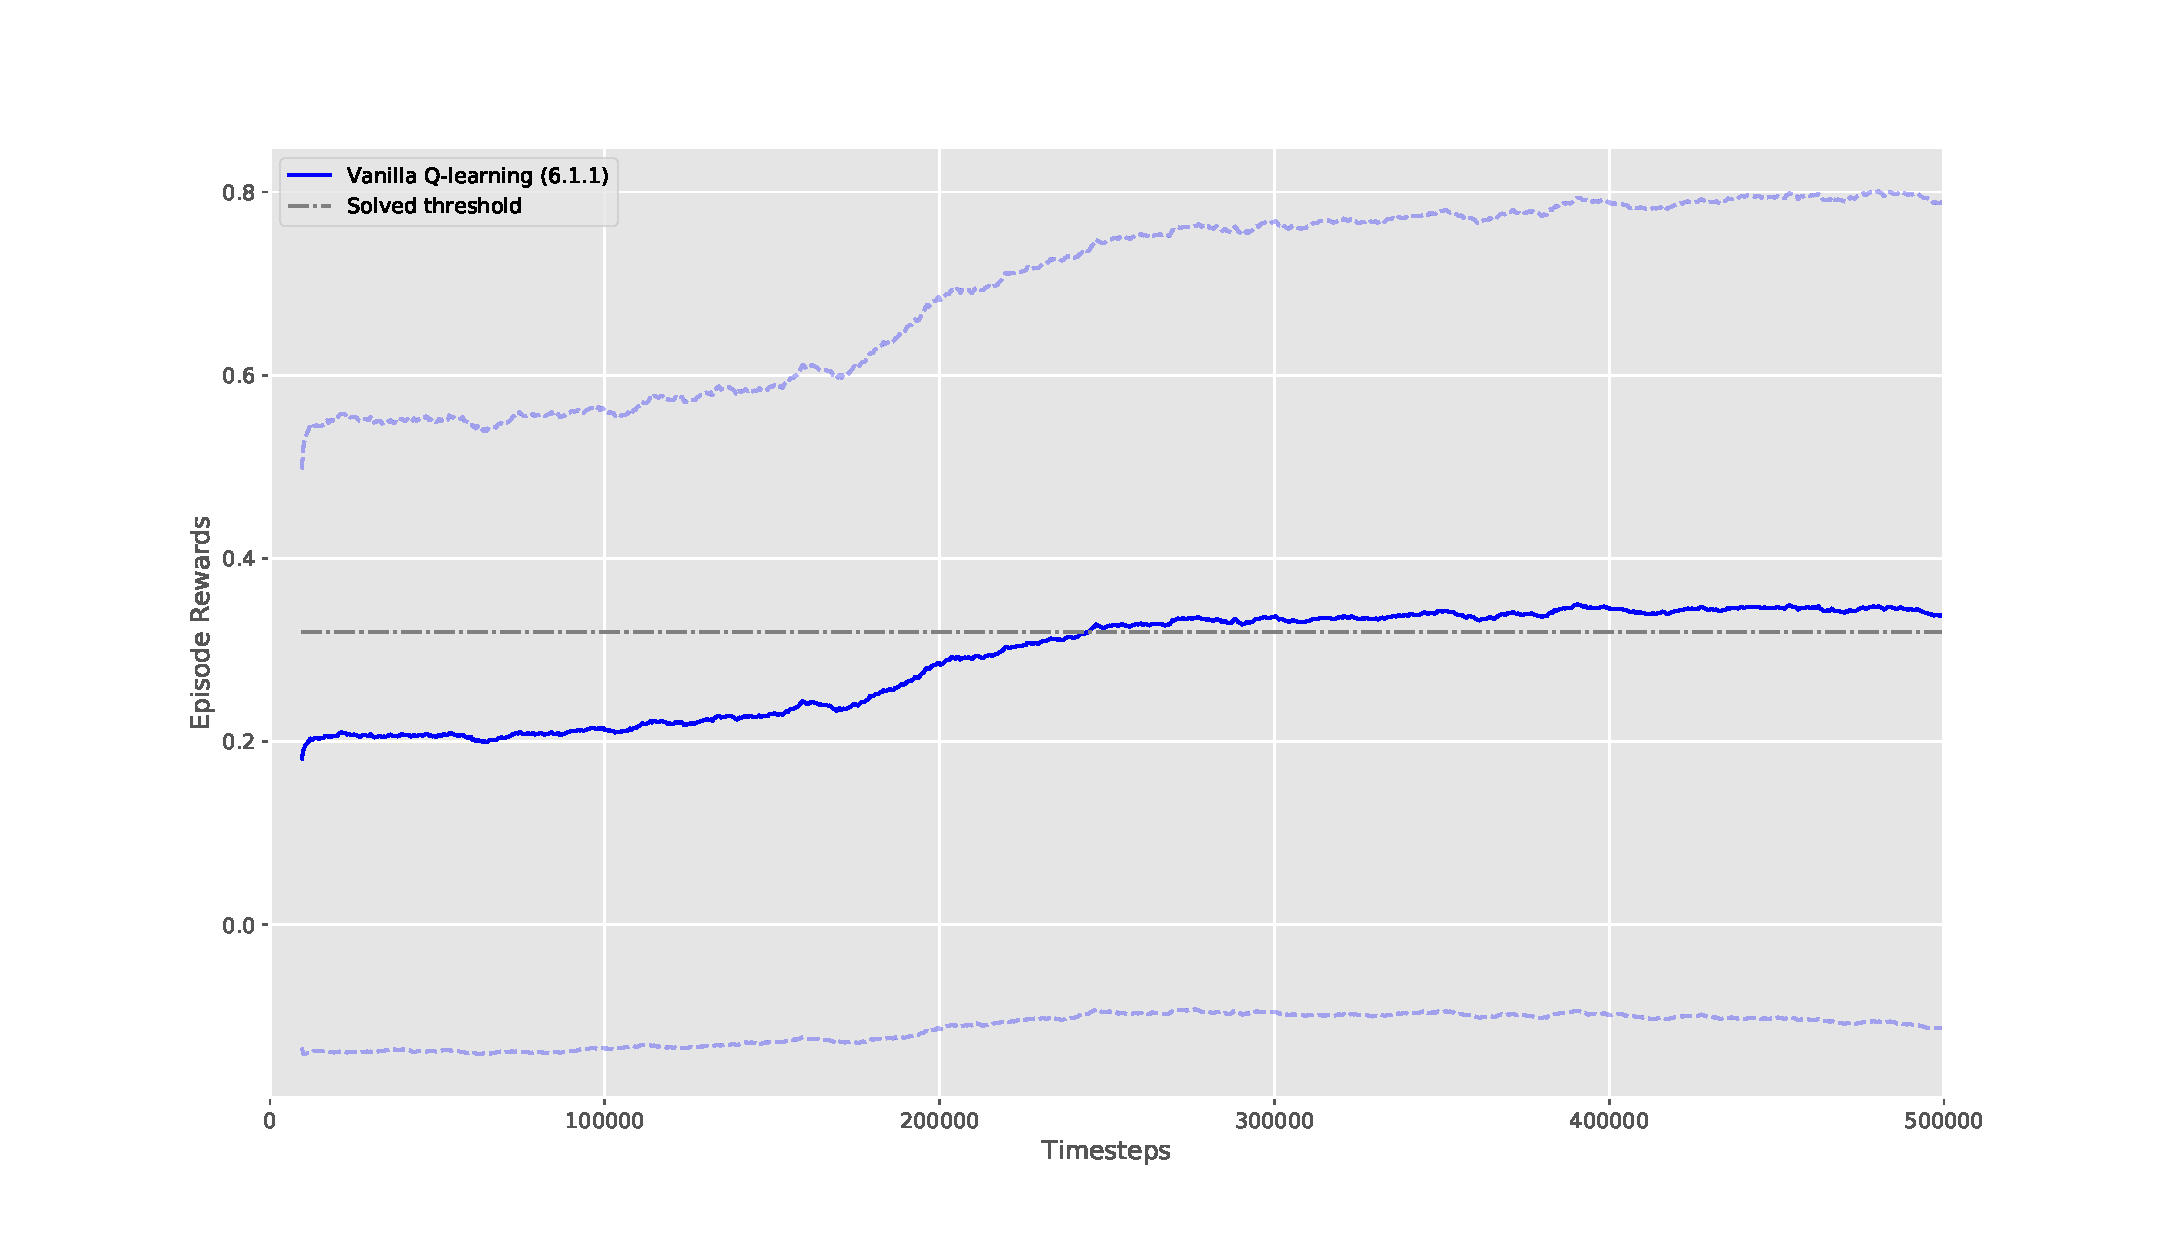
\includegraphics[width=15cm]{Figures/QlearningBaselineBench}
\caption{Vanilla Q-learning: Rewards over timesteps}
\label{fig:QlearningBaselineBench}
\end{figure}


\section{Discriminator techniques}


\subsection{Update whole Q-table (Approach \ref{ssec:QlearningGANWhole})}
Figure~\ref{fig:QlearningGANWholeBench} shows the results of the model that we presented in section 6.1.2, which updates the whole Q-table after each timestep (magenta plot). 
We also include both baselines: the model trained with vanilla Q-learning (blue) and the model that uses L2 regularisation towards the average of the training Q-tables (orange).
As usual, we plot the standard deviations of all models.
We notice how vanilla Q-learning performs better than these two models that use transfer learning.
We motivate this poor performance on the fact that update the whole Q-table can throw off vanilla Q-learning and the $\epsilon$-greedy approach fails to recover after each inaccurate update towards the gradient of the discriminator.

Our method, while being less efficient than Q-learning in terms of the average rewards obtained on the test domains, nevertheless manages to solve the domain after an average of 430,000 timesteps, which is still much higher than the 250,000 timesteps of vanilla Q-learning.

\begin{figure}[H]
\centering
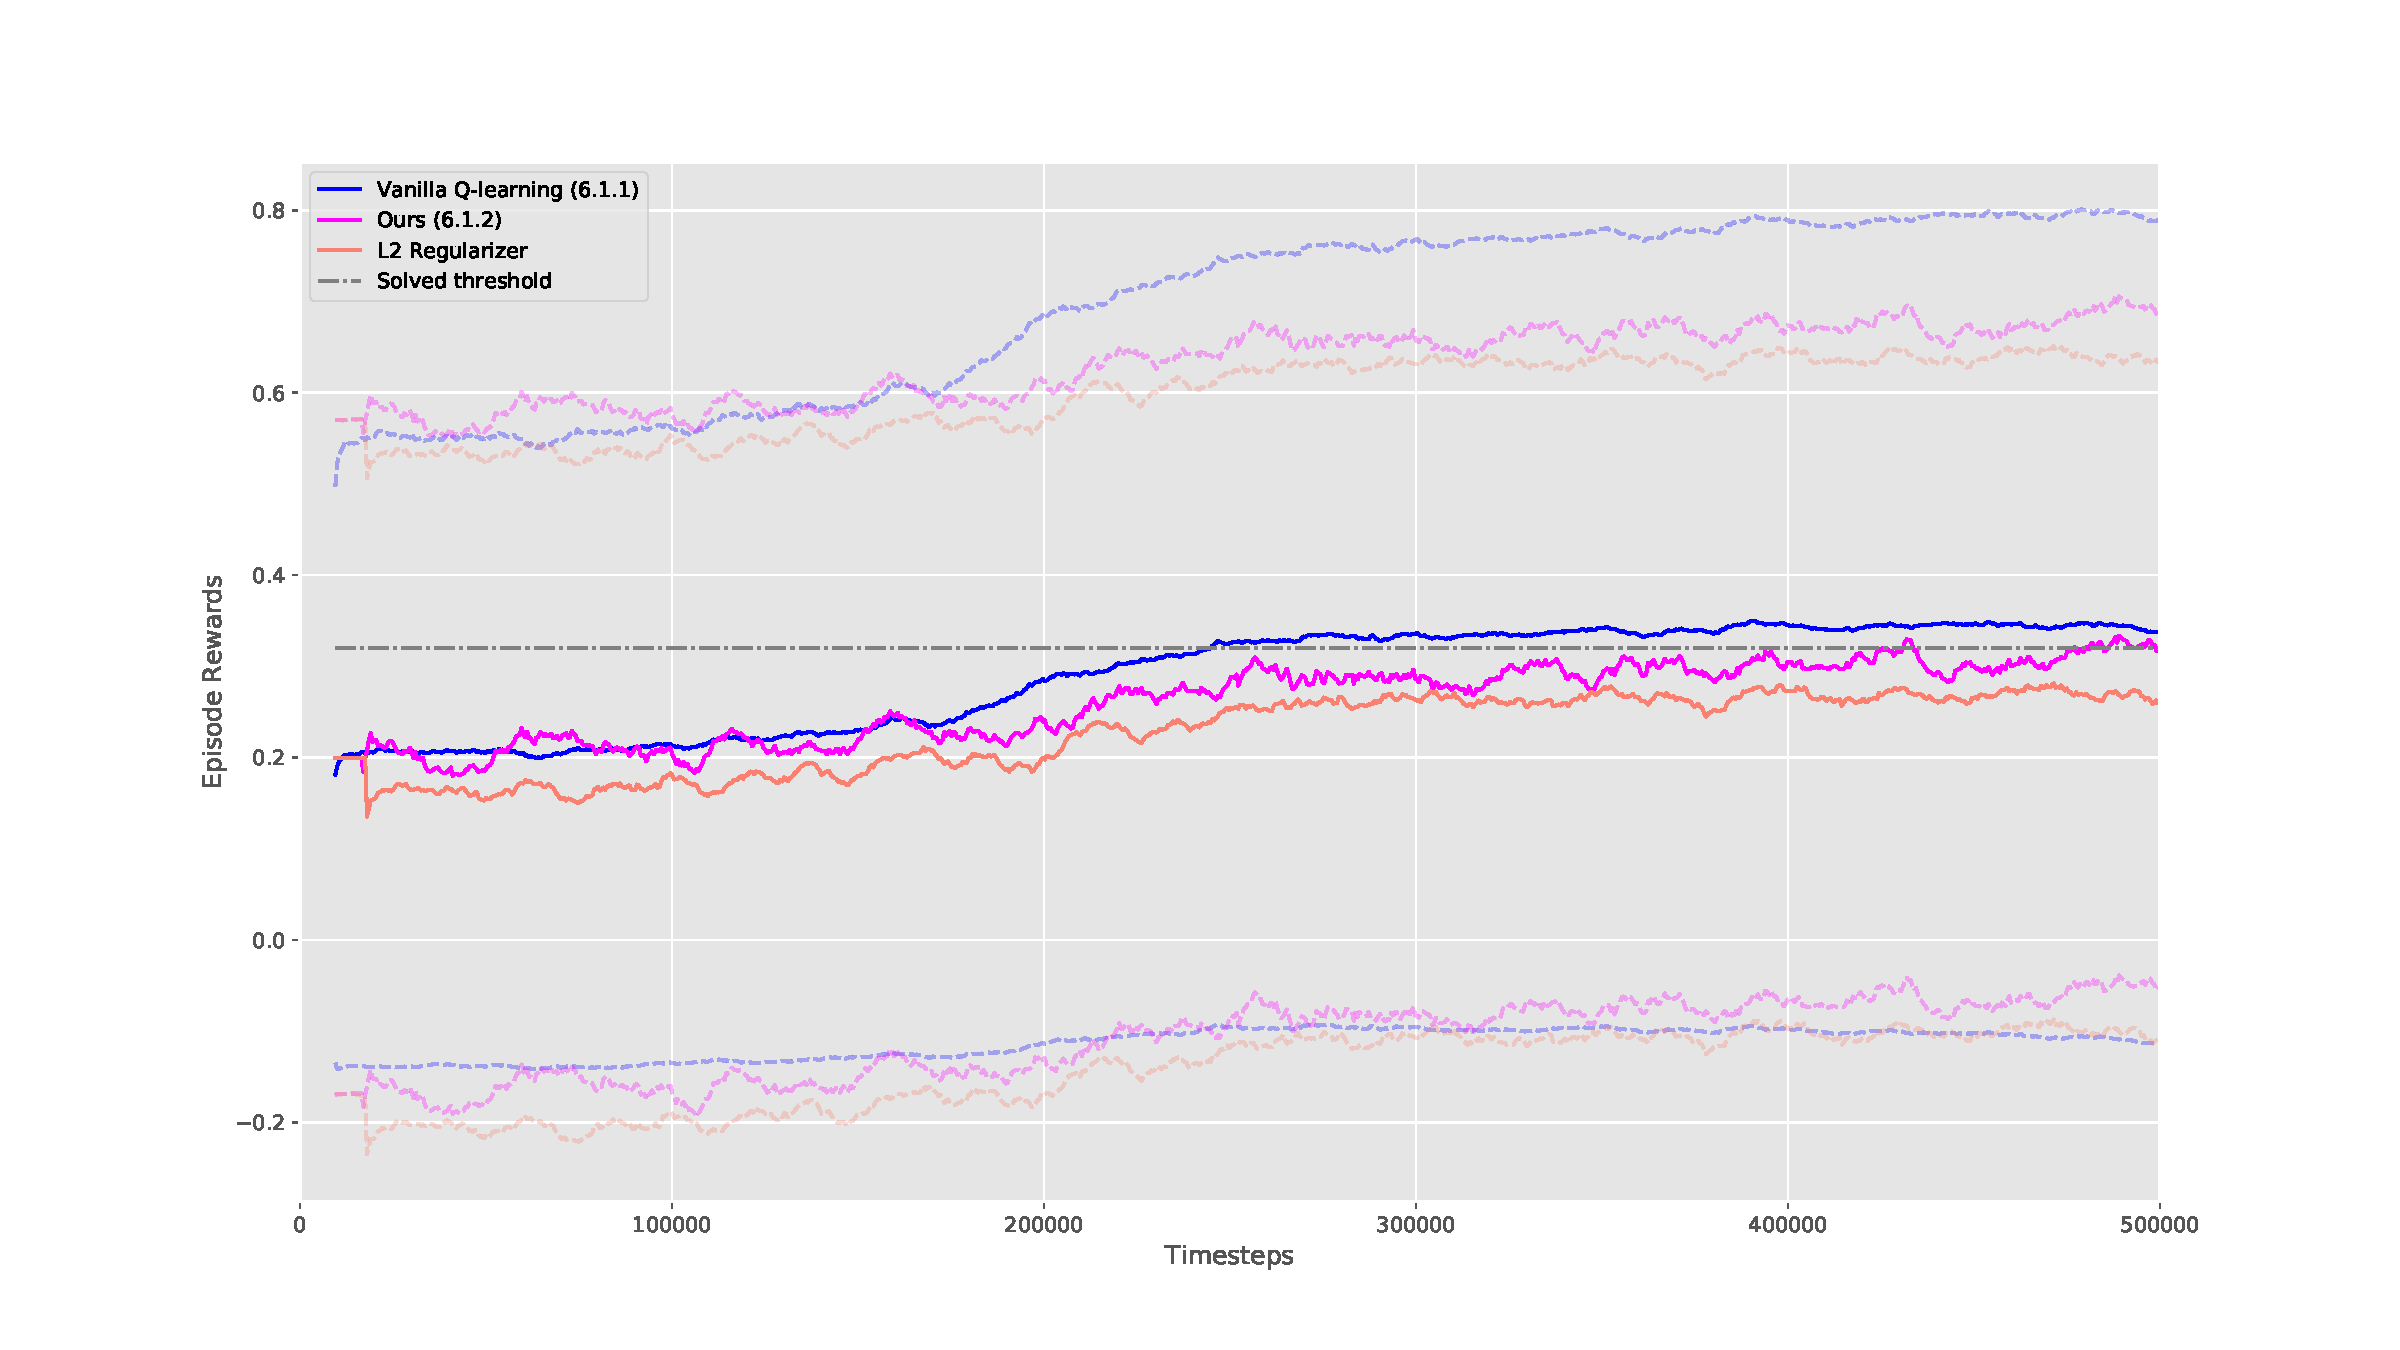
\includegraphics[width=15cm]{Figures/QlearningGANWholeBench}
\caption{Q-learning with whole Q-table: Rewards over timesteps}
\label{fig:QlearningGANWholeBench}
\end{figure}


\subsection{Update Q-table pair (Approach \ref{ssec:QlearningGANPair})}
Figure~\ref{fig:QlearningGANPairBench} shows the results of the transfer learning approach whereby instead of updating the whole Q-table towards the direction of $\nabla D(Q_{t})$, we update only the state/action pair in that particular timestep.

\begin{figure}[H]
\centering
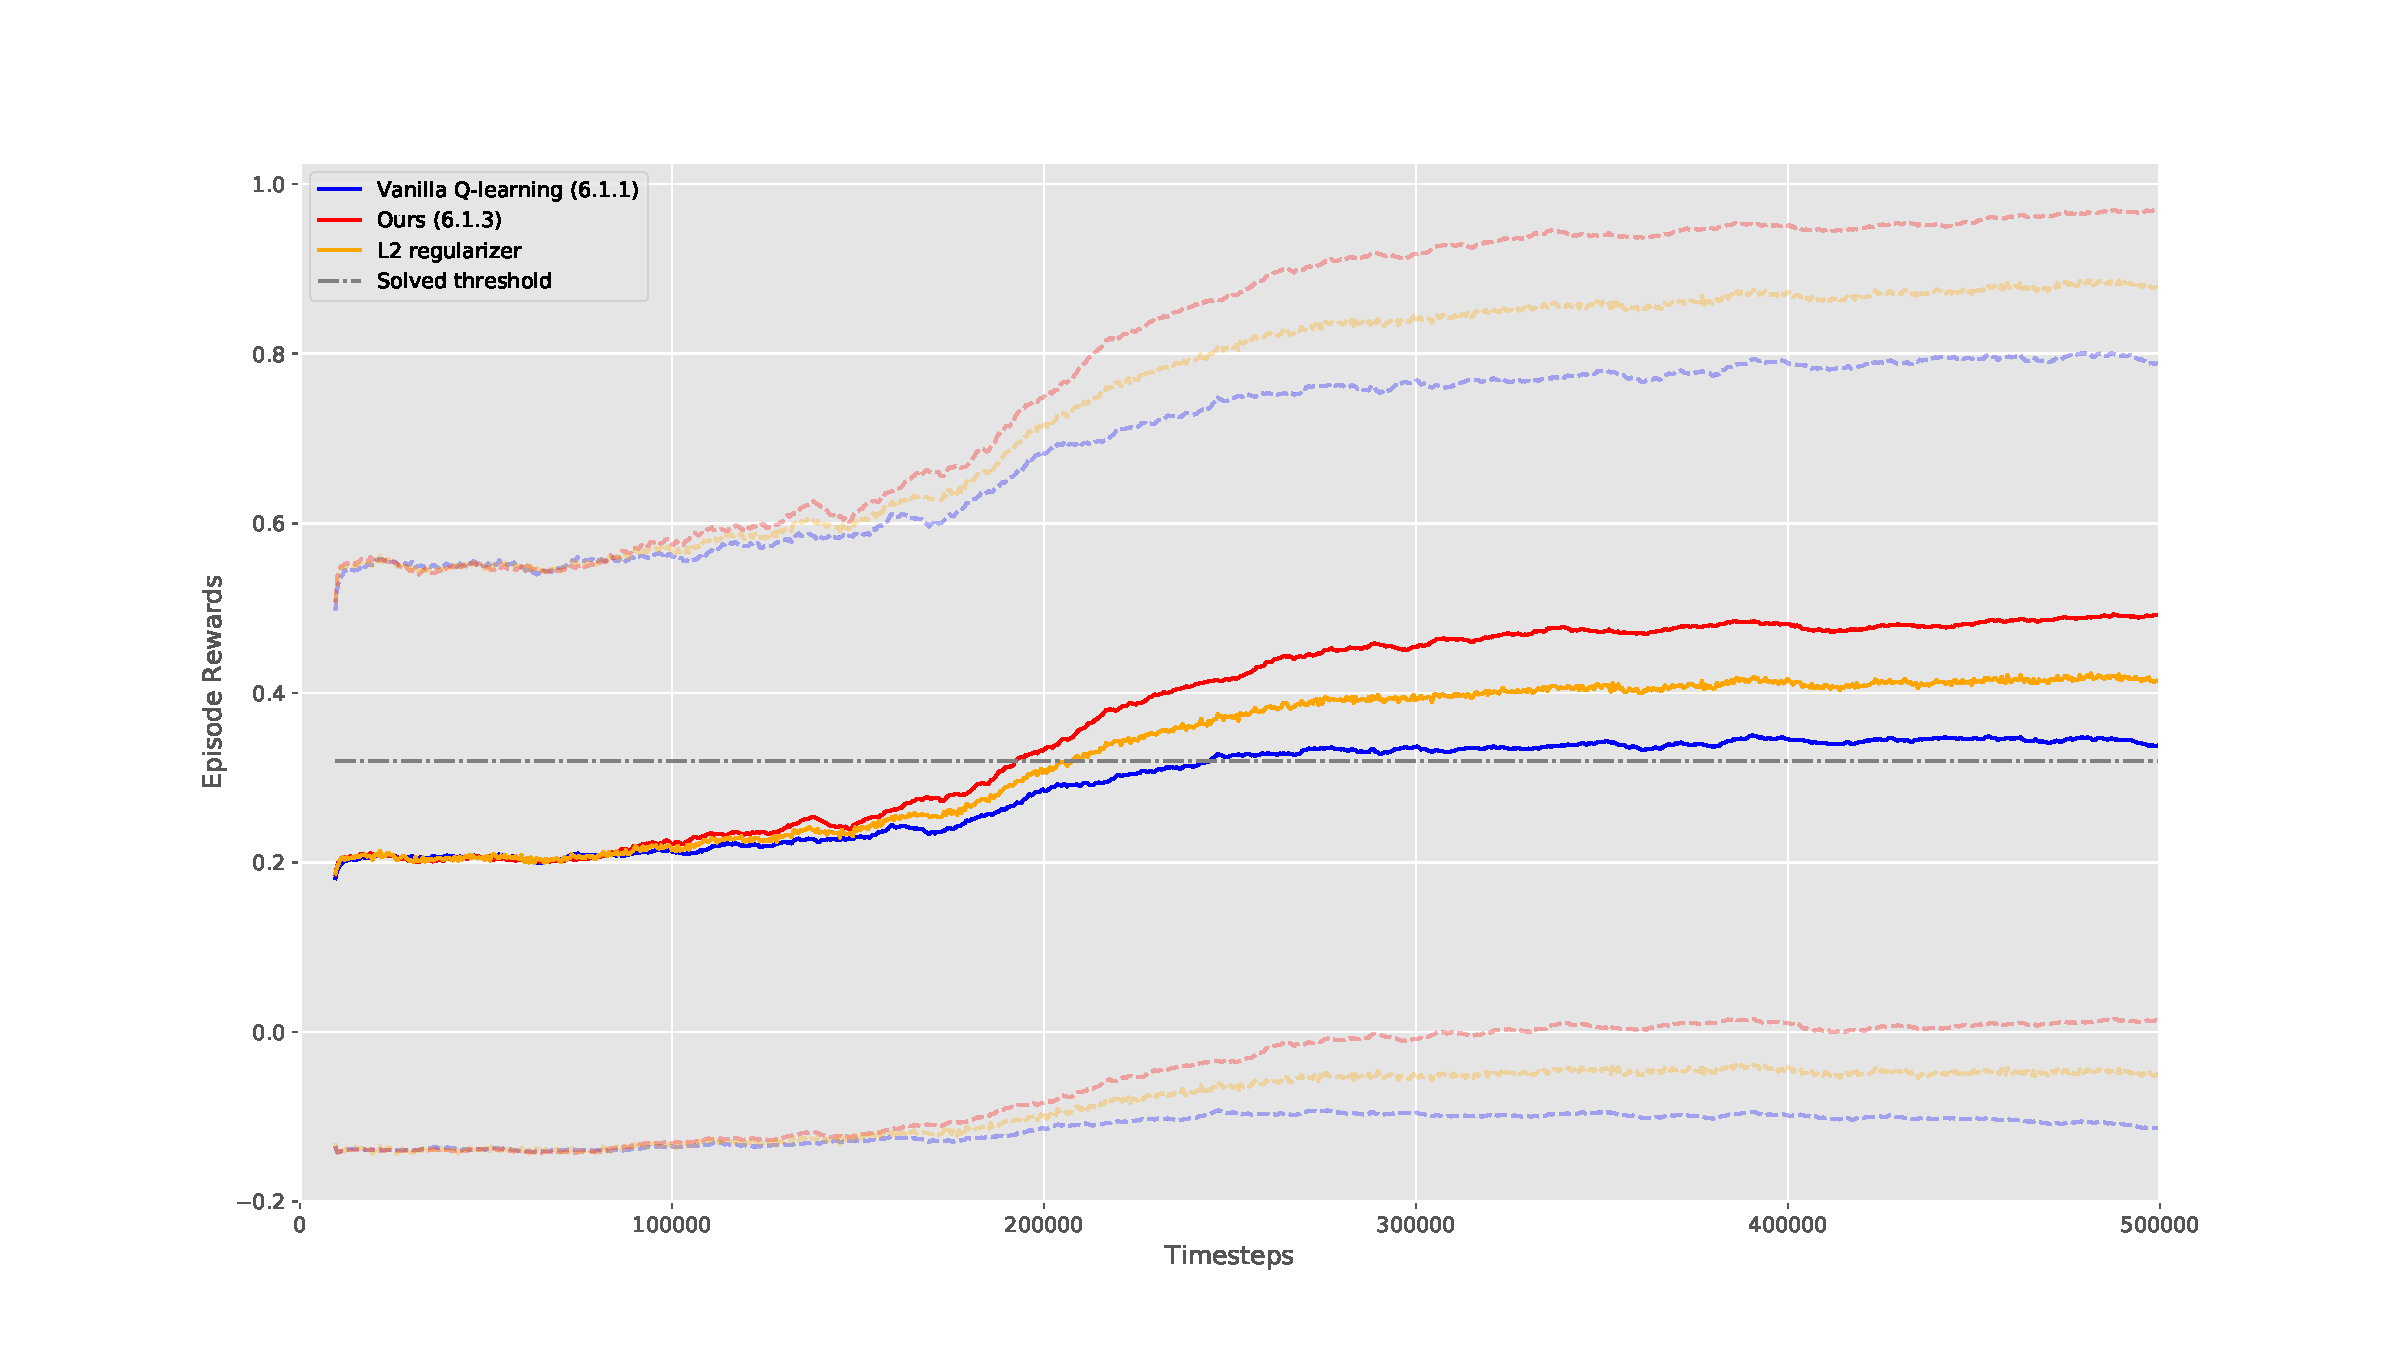
\includegraphics[width=15cm]{Figures/QlearningGANPairBench}
\caption{Q-learning with state/action pair update: Rewards over timesteps}
\label{fig:QlearningGANPairBench}
\end{figure}

We see right away that our model (red plot) asymptotically achieves much higher average rewards than our baseline models. We solve the task at just over 190,000 timesteps by reaching our reward threshold  of 0.32 much earlier than our baseline models.

Just like in the previous benchmark, here we also take into account the model with L2 regularisation towards the mean of the test set as one of our baseline. However, instead of again updating the whole table, we update the corresponding state/action value in the Q-table. We see that while that performs better than vanilla Q-learning, the discriminative model trained with the GAN is better able to capture transferrable information to feed back to the iterative Q-table update. 


\subsection{Update Q-table row (Approach \ref{ssec:QlearningGANRow})}
This approach is not as conservative as the previous one, as it updates the whole row of the state the agent is in after each timestep.

This model also performs better than both baselines, solving the task after an average of 210,000 timesteps.

Once again, the L2 regulariser baseline only pushes the appropriate row towards the mean Q-tables, rather than the whole table.

\begin{figure}[H]
\centering
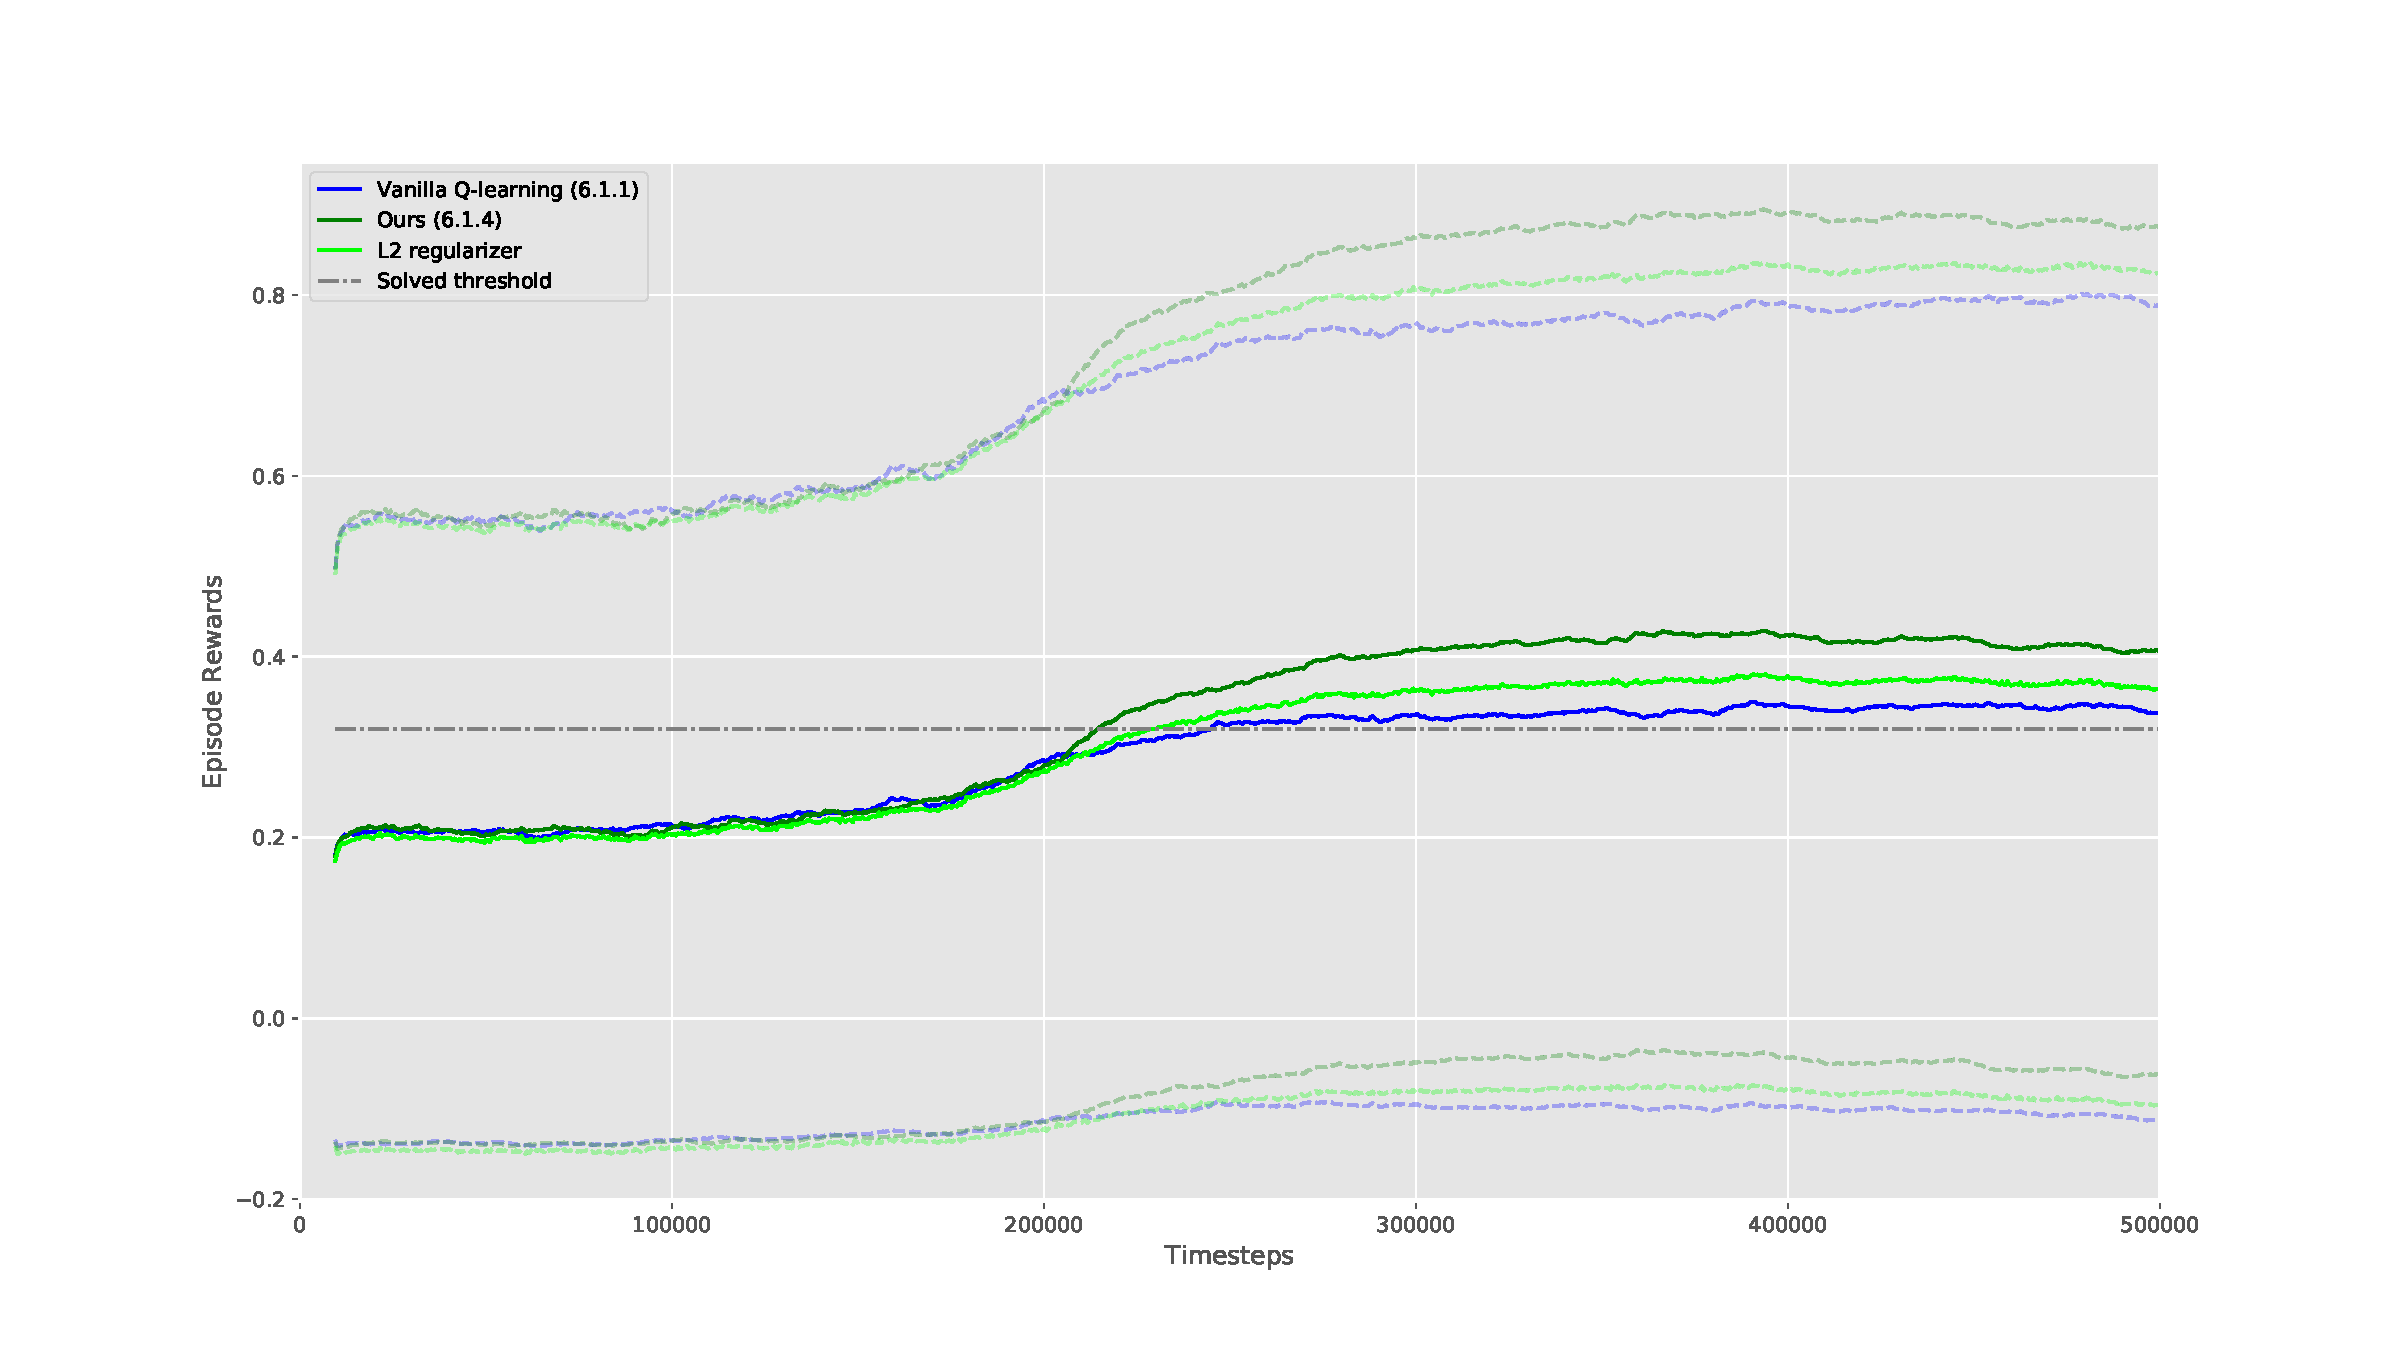
\includegraphics[width=15cm]{Figures/QlearningGANRowBench}
\caption{Q-learning with row update: Rewards over timesteps}
\label{fig:QlearningGANRowBench}
\end{figure}

\subsection{Discriminator benchmarks overview}
Here in figure~\ref{fig:QlearningGANAllDiscrim} we display the overall results of our transfer learning techniques compared to the vanilla Q-learning results. Table~\ref{tab:aucdiscrim} reports in descending order the area under the curve metric (AuC) of each average reward plot. We can use this metric to measure the overall cumulative rewards during training. In combination with the reward threshold line, we can have through these two metrics a summative overview of how our models are performing when transferring knowledge.

\begin{figure}[H]
\centering
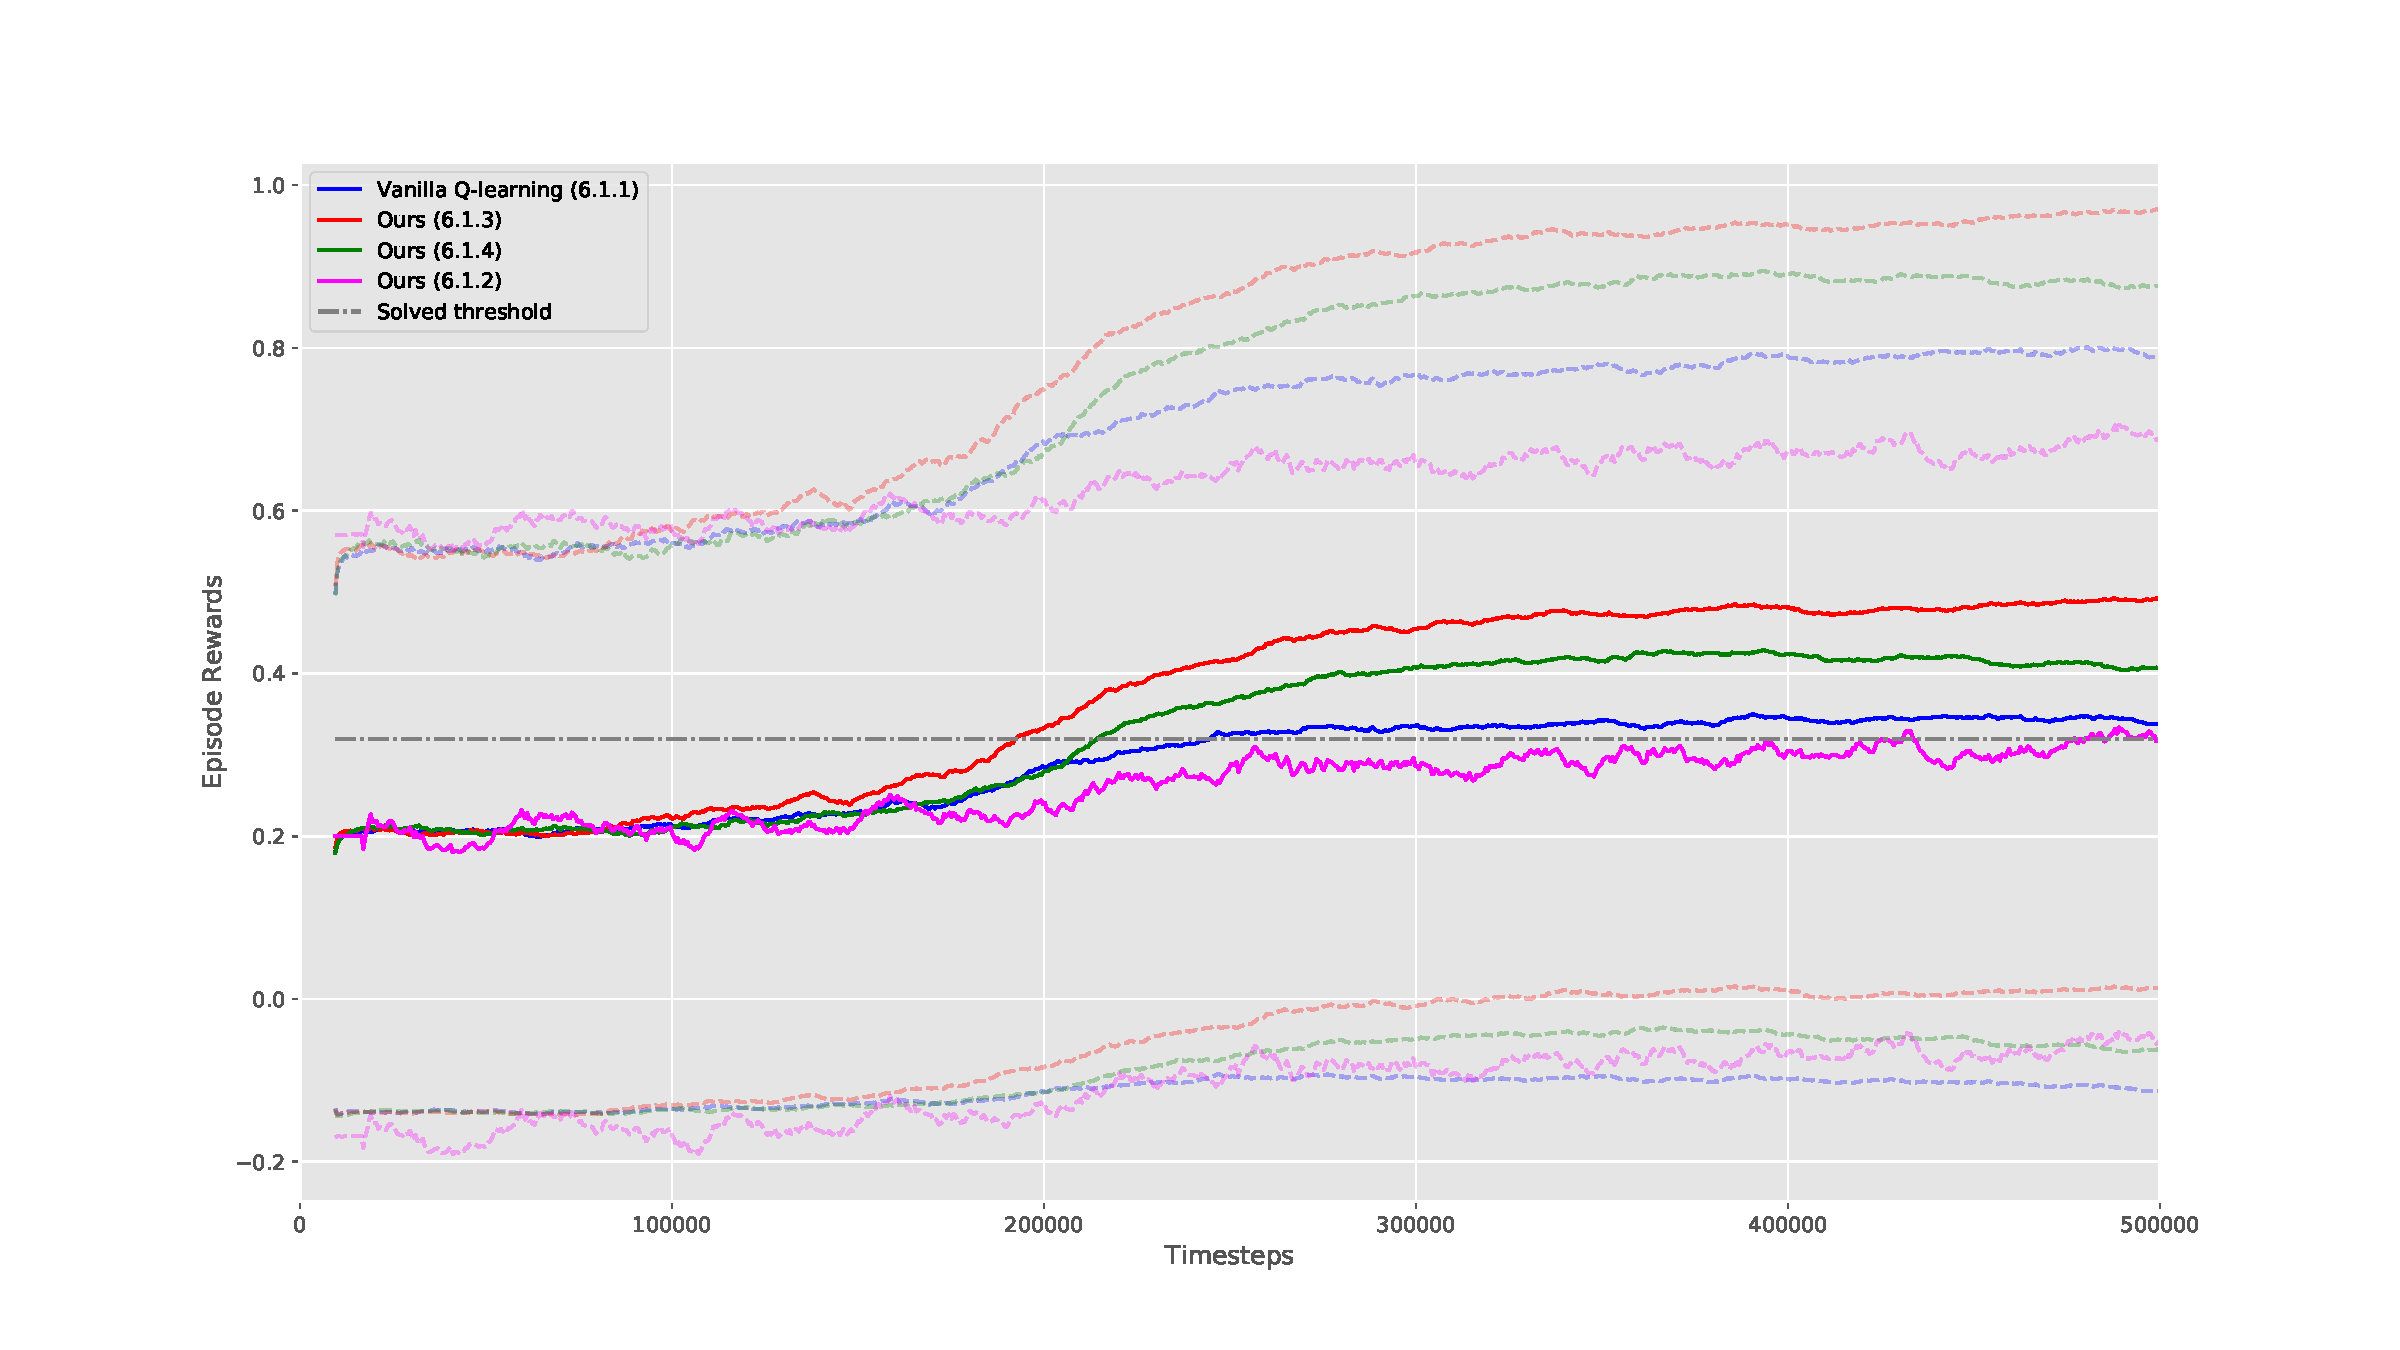
\includegraphics[width=15cm]{Figures/QlearningGANAllDiscrim}
\caption{Q-learning with state/action pair update: Rewards over timesteps}
\label{fig:QlearningGANAllDiscrim}
\end{figure}


\begin{table}[H]
\centering
\begin{tabular}{@{}ll@{}}
\toprule
Transfer learning approach & AuC     \\ \midrule
Q-table state/pair update (approach~\ref{ssec:QlearningGANPair})  & 1816.29 \\
Q-table row update (approach~\ref{ssec:QlearningGANRow})        & 1615.63 \\
Vanilla GAN (baseline)     & 1420.80 \\
Whole Q-table update (approach~\ref{ssec:QlearningGANWhole})      & 1282.46 \\ \bottomrule
\end{tabular}
\caption{Area under the curve of different approaches in descending order of AuC}
\label{tab:aucdiscrim}
\end{table}

\section{Generator techniques}
\subsection{Global search (approach~\ref{ssec:globalsearch})}
With the global search technique, we directly sample Q-tables from the generator to use as policies for the task at hand. Thus, there is no direct training process in the sense of iterative Q-table updates.

The only fixed hyperparameter in this approach is the number of sampled Q-tables from the Generator network, from which we will pick the one that yields the best results in terms of rewards. This number great affects the runtime of the algorithm, as we need to check the rewards for each policy.

To find a good compromise between number of sampled policies and its performance on the test set, we build table~\ref{tab:avgrewardsglobalsearch}.

It is clear from this, that even by sample 100,000 policies, on average, the best policies do not perform as well as the baseline policies trained with vanilla Q-learning, which, as we saw in section~\ref{sec:metricsbaselinemodel} achieved an asymptotic average reward of 0.36, much more than the maximum of 0.2932 we achieve with global search.

It is still worth to reiterate that global search may still return good policies with domains that have a relatively small policy space.

\begin{table}[H]
\centering
\begin{tabular}{@{}ll@{}}
\toprule
\# sampled Q-tables/policies & Avg rewards test set \\ \midrule
1                            & 0.2123               \\
10                           & 0.2738               \\
1,000                        & 0.2801               \\
5,000                        & 0.2832               \\
10,000                       & 0.2902               \\
100,000                      & 0.2932               \\ \bottomrule
\end{tabular}
\caption{Average rewards in test set tasks for different number of sampled Q-tables/policies from the Generator}
\label{tab:avgrewardsglobalsearch}
\end{table}

\subsection{Global/local search (approach~\ref{ssec:localglobalsearch})}
The global/local search hybrid approach, we take in the best Q-table/policy found with global search, and use that Q-table as the starting point of our training.  We could use any technique from the previous section for local search, but to greatly limit the number of experiments that we need to run, we pick the model that performed best in our discriminator benchmarks earlier. That is approach~\ref{ssec:QlearningGANPair} where we update a single state/action pair from $\nabla D(Q_{t})$.

Table~\ref{tab:avgrewardslocalglobalsearch} shows the asymptotic performance after local search of each model when taking increasing number of sampled policies.

\begin{table}[H]
\centering
\begin{tabular}{@{}ll@{}}
\toprule
\# sampled Q-tables/policies & Avg rewards test set \\ \midrule
1                            & 0.5223               \\
10                           & 0.5238               \\
1,000                        & 0.5401               \\
5,000                        & 0.5632               \\
10,000                       & 0.5702               \\
100,000                      & 0.5712               \\ \bottomrule
\end{tabular}
\caption{Average rewards in test set tasks for different number of sampled Q-tables/policies from the Generator}
\label{tab:avgrewardslocalglobalsearch}
\end{table}

An optimal number of policies to sample seems to 10,000 for our environment setup, but it may vary for different domains and the result generally depends, particularly at lower number of sample Q-tables, on how fortuitous we are with the Q-tables that we sample from the Generator network.

Finally, figure~\ref{fig:globallocalsearchBench} shows the plot of the model when we take 10,000 sampled policies during local search. From this figure we notice a few things:
\begin{enumerate}
	\item The global/local search policy reaches the reward threshold earlier than our best model before.
	\item The overall rewards (i.e. AuC) will also be slightly better.
	\item The starting point derived from global search allows us to have better rewards even at earlier timesteps.
\end{enumerate}

\begin{figure}[H]
\centering
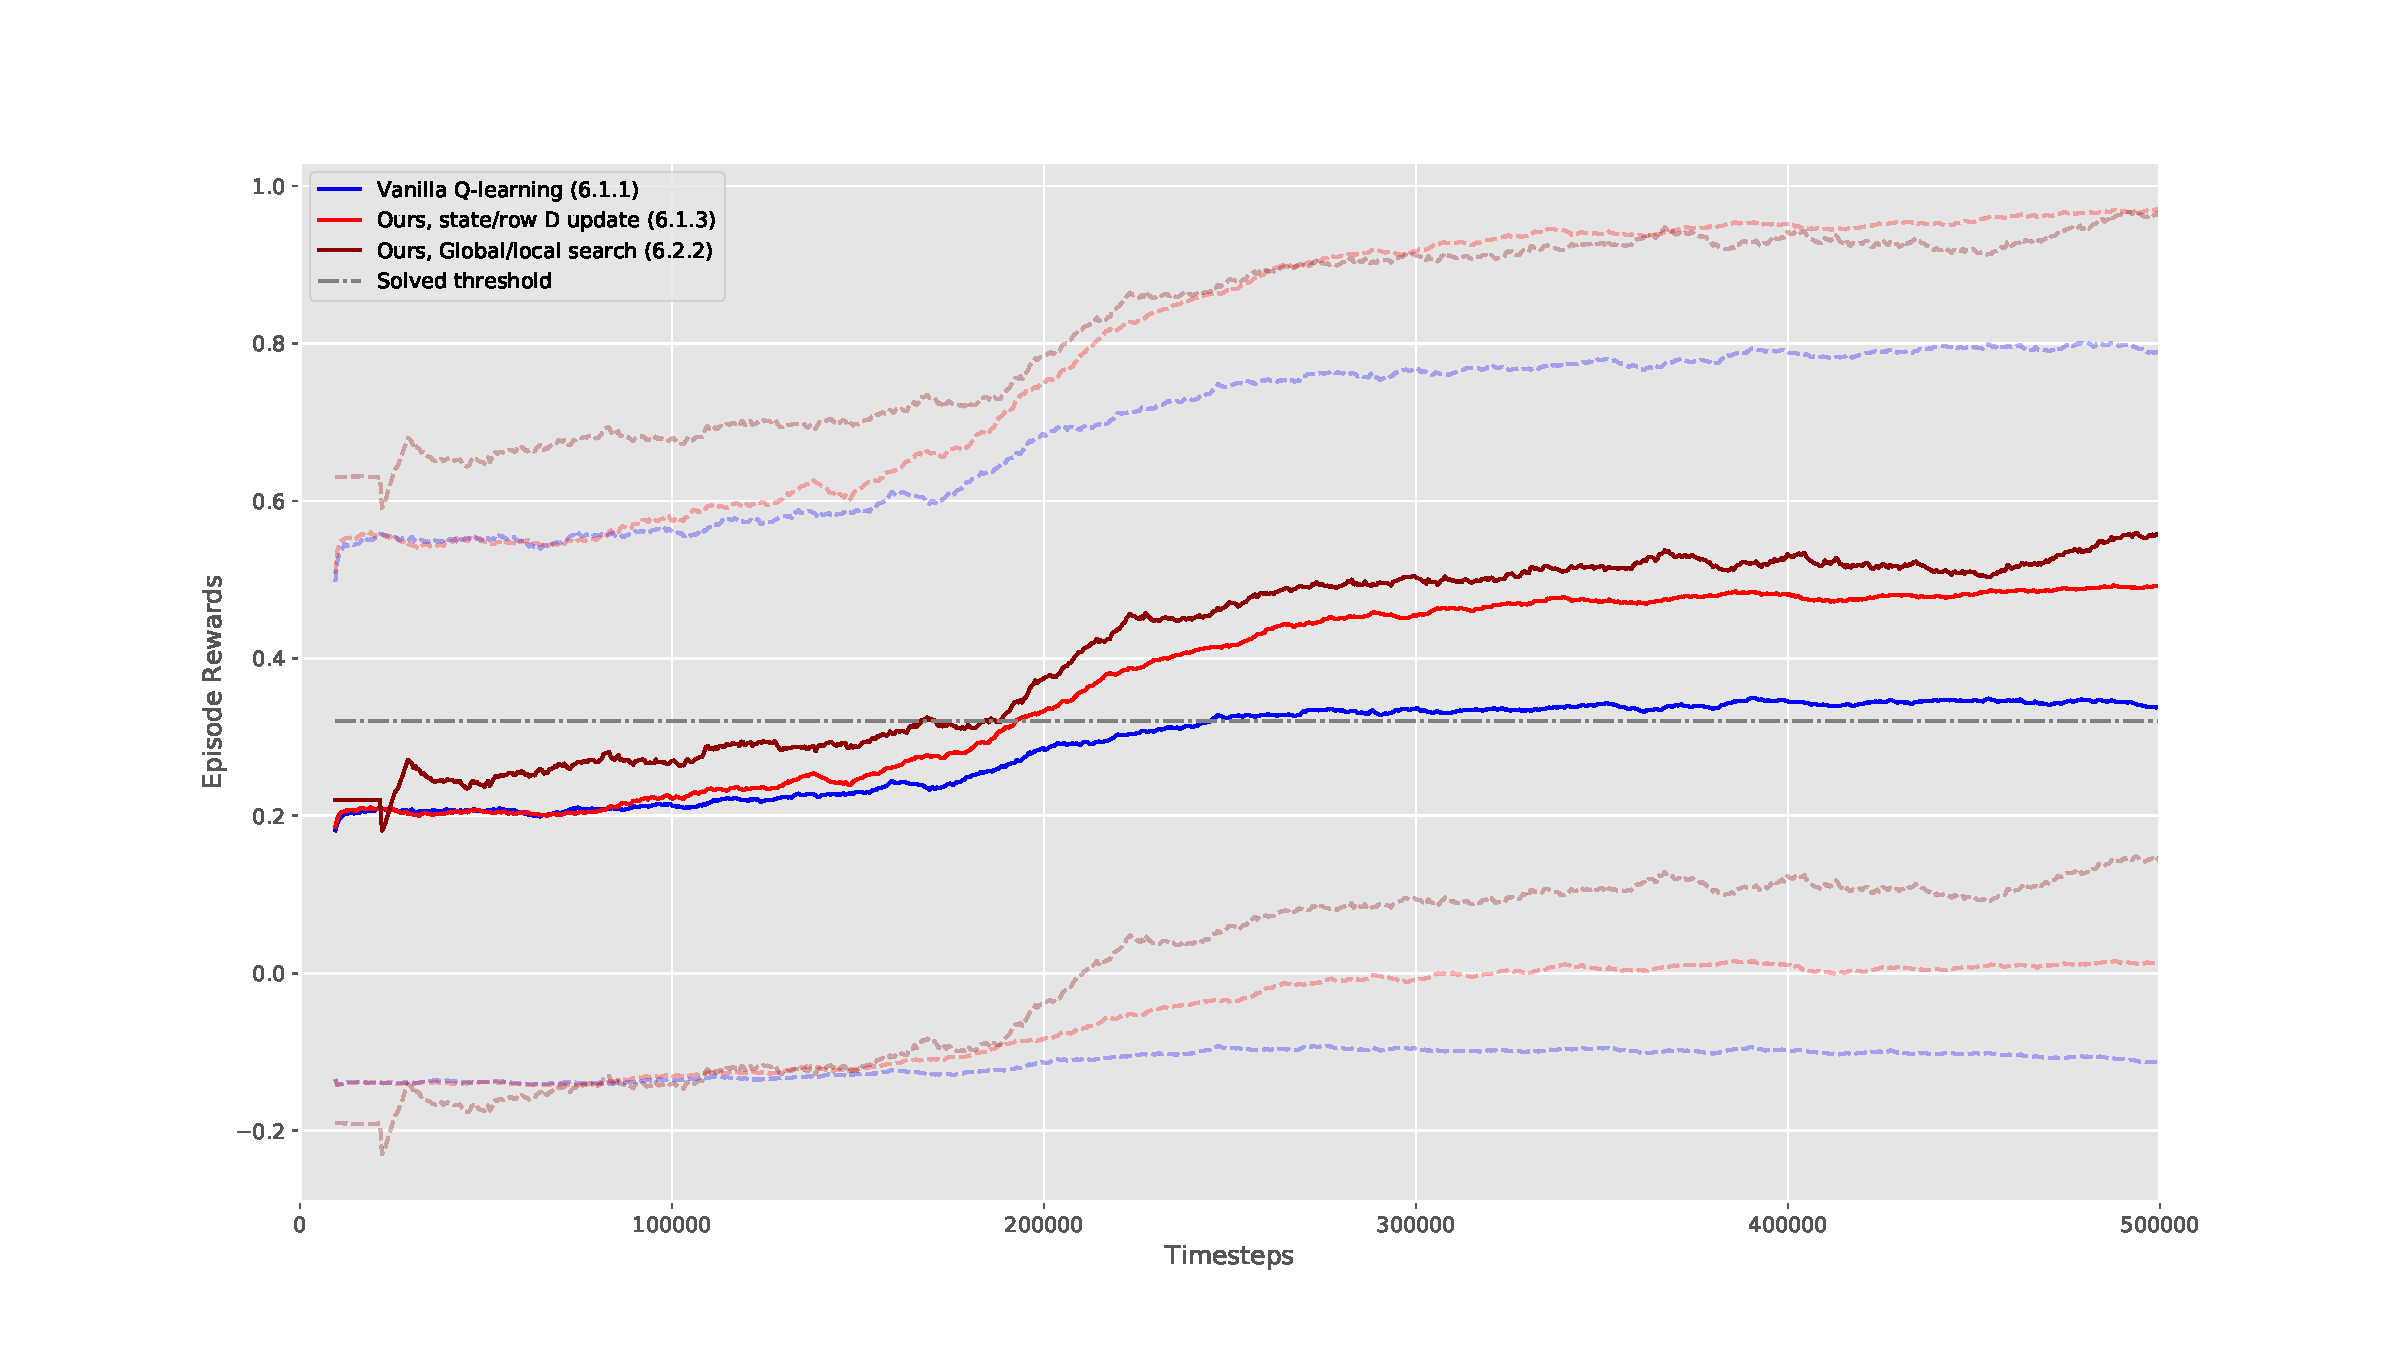
\includegraphics[width=15cm]{Figures/globallocalsearchBench}
\caption{Q-learning with state/action pair update: Rewards over timesteps}
\label{fig:globallocalsearchBench}
\end{figure}

\begin{table}[H]
\centering
\begin{tabular}{@{}ll@{}}
\toprule
Transfer learning approach & AuC     \\ \midrule
Global/local search (approach~\ref{ssec:localglobalsearch})  & 2028.64 \\
Q-table state/pair update (approach~\ref{ssec:QlearningGANPair})  & 1816.29 \\
Vanilla GAN (baseline)     & 1420.80 \\
\end{tabular}
\caption{Area under the curve of different approaches in descending order of AuC}
\label{tab:aucgenerator}
\end{table}

% Chapter 8

\chapter{Conclusion} % Main chapter title

\label{Chapter8} % For referencing the chapter elsewhere, use \ref{Chapter1} 

%----------------------------------------------------------------------------------------
%	THESIS CONTENT - APPENDICES
%----------------------------------------------------------------------------------------

\appendix % Cue to tell LaTeX that the following "chapters" are Appendices

% Include the appendices of the thesis as separate files from the Appendices folder
% Uncomment the lines as you write the Appendices

%% Appendix A

\chapter{Frequently Asked Questions} % Main appendix title

\label{AppendixA} % For referencing this appendix elsewhere, use \ref{AppendixA}

\section{How do I change the colors of links?}

The color of links can be changed to your liking using:

{\small\verb!\hypersetup{urlcolor=red}!}, or

{\small\verb!\hypersetup{citecolor=green}!}, or

{\small\verb!\hypersetup{allcolor=blue}!}.

\noindent If you want to completely hide the links, you can use:

{\small\verb!\hypersetup{allcolors=.}!}, or even better: 

{\small\verb!\hypersetup{hidelinks}!}.

\noindent If you want to have obvious links in the PDF but not the printed text, use:

{\small\verb!\hypersetup{colorlinks=false}!}.

%\include{Appendices/AppendixB}
%\include{Appendices/AppendixC}

%----------------------------------------------------------------------------------------
%	BIBLIOGRAPHY
%----------------------------------------------------------------------------------------

\printbibliography[heading=bibintoc]

%----------------------------------------------------------------------------------------

\end{document}  
